% ****** Start of file apssamp.tex ******
%
%   This file is part of the APS files in the REVTeX 4.1 distribution.
%   Version 4.1r of REVTeX, August 2010
%
%   Copyright (c) 2009, 2010 The American Physical Society.
%
%   See the REVTeX 4 README file for restrictions and more information.
%
% TeX'ing this file requires that you have AMS-LaTeX 2.0 installed
% as well as the rest of the prerequisites for REVTeX 4.1
%
% See the REVTeX 4 README file
% It also requires running BibTeX. The commands are as follows:
%
%  1)  latex apssamp.tex
%  2)  bibtex apssamp
%  3)  latex apssamp.tex
%  4)  latex apssamp.tex
%
%\documentclass[aps,prb,showpacs,amsmath,amssymb,superscriptaddress]{revtex4-1}
\documentclass[prf,superscriptaddress,showpacs]{revtex4-1}

%\documentclass[%
%reprint,
%superscriptaddress,
%groupedaddress,
%unsortedaddress,
%runinaddress,
%frontmatterverbose, 
%preprint,
%showpacs,preprintnumbers,
%nofootinbib,
%nobibnotes,
%bibnotes,
 %amsmath,amssymb,
 %aps,
%pra,
%prb,
%rmp,
%prstab,
%prstper,
%floatfix,
%]{revtex4-1}

\usepackage{amsmath,amssymb}
\usepackage[titletoc]{appendix}
\usepackage{todonotes}
\usepackage{graphicx}% Include figure files
\usepackage{dcolumn}% Align table columns on decimal point
\usepackage{bm}% bold math
\usepackage{stmaryrd}
%\usepackage{hyperref}% add hypertext capabilities
%\usepackage[mathlines]{lineno}% Enable numbering of text and display math
%\linenumbers\relax % Commence numbering lines

%\usepackage[showframe,%Uncomment any one of the following lines to test 
%%scale=0.7, marginratio={1:1, 2:3}, ignoreall,% default settings
%%text={7in,10in},centering,
%%margin=1.5in,
%%total={6.5in,8.75in}, top=1.2in, left=0.9in, includefoot,
%%height=10in,a5paper,hmargin={3cm,0.8in},
%]{geometry}

\renewcommand{\AA}{\mathcal{A}}
\newcommand{\BB}{\mathcal{B}}
\newcommand{\DD}{\mathcal{D}}
\newcommand{\ff}{\mathbf{f}}
\newcommand{\nn}{\mathbf{n}}
\renewcommand{\tt}{\mathbf{t}}
\newcommand{\pderiv}[2]{\frac{\partial #1}{\partial #2}}
\newcommand{\rr}{\mathbf{r}}
\newcommand{\RR}{\mathbb{R}}
\renewcommand{\ss}{\mathbf{s}}
\renewcommand{\SS}{\mathcal{S}}
\newcommand{\TT}{\mathcal{T}}
\newcommand{\uu}{\mathbf{u}}
\newcommand{\WW}{\mathcal{W}}
\newcommand{\xx}{\mathbf{x}}
\newcommand{\xxi}{\boldsymbol{\xi}}
\newcommand{\yy}{\mathbf{y}}

\begin{document}

\preprint{APS/123-QED}

\title{Hydrodynamics and rheology of adhesive vesicle doublets}
% Force line breaks with \\
%\thanks{A footnote to the article title}%

\author{Bryan Quaife}
\affiliation{Department of Scientific Computing, Florida State University, Tallahassee, Florida, USA}
% \email{bquaife@fsu.edu}
\author{Shravan Veerapaneni}%
% \email{shravan@umich.edu}
\affiliation{Department of Mathematics, University of Michigan, Ann Arbor, Michigan, USA}%
\author{Y.-N.~Young}%
 \email[Corresponding author: ]{yyoung@njit.edu}
\affiliation{Department of Mathematical Sciences, Newark, NJ, USA}%

\date{\today}% It is always \today, today,
             %  but any date may be explicitly specified

\begin{abstract}
The dynamics of an adhesive vesicle doublet under various flow conditions is
investigated numerically using a high-order, adaptive-in-time boundary
integral method. In a quiescent flow, two nearby vesicles
move slowly towards each other under the adhesive potential, pushing out
fluid between them to form a vesicle doublet at equilibrium. A lubrication
analysis on such draining of a thin film gives the dependencies of
draining time on adhesion strength and separation distance that are in
good agreement with numerical results.
%
In a microfluid trap where the stagnation of an extensional flow is dynamically
placed in the middle of a vesicle doublet through an active control
loop, novel dynamics of a vesicle doublet is observed. Numerical
simulations show that there exists a critical extensional flow rate
above which adhesive interaction is overcome by the 
diverging stream, thus providing a simple method to measure the adhesion
strength between two vesicle membranes. 
%
In a planar shear flow, numerical simulations reveal that a vesicle
doublet may form as two vesicles approach each other provided that the adhesion
strength is sufficiently large at a given vesicle reduced area. Once a
doublet is formed, the effective shear viscosity of a dilute suspension
of vesicle doublets is found to be a function of both reduced area and
the adhesion strength.  Results from these numerical studies and
analysis shed light on the hydrodynamic effects of adhesive interactions
between vesicles in a viscous fluid.
%\begin{description}
%\item[Usage]
%Secondary publications and information retrieval purposes.
%\item[PACS numbers]
%May be entered using the \verb+\pacs{#1}+ command.
%\item[Structure]
%You may use the \texttt{description} environment to structure your abstract;
%use the optional argument of the \verb+\item+ command to give the category of each item. 
%\end{description}
\end{abstract}

\pacs{Valid PACS appear here}% PACS, the Physics and Astronomy
                             % Classification Scheme.
%\keywords{Suggested keywords}%Use showkeys class option if keyword
                              %display desired
\maketitle

%\tableofcontents

%%%%%%%%%%%%%%%%%%%%%%%%%%%%%%%%%%%%%%%%%%%%%%%%%%%%%%%%%%%%%%%%%%%%%%%%

\section{Introduction}
Vesicles (closed fluid-filled phospholipid bilayer membranes) have been
widely utilized as biological cell mimics in biophysics and material
engineering~\cite{sackmann1996, Barthes-Biesel2016_ARFM}.  The ever
expanding applications have encouraged detailed experimental,
theoretical and numerical investigations of vesicle hydrodynamics in
applied flow, electric and magnetic fields.  Theoretical
investigations often take the form of small-deformation analysis or
spheroidal dynamics of a nearly-spherical vesicle (or nearly-circular in
two dimensions) subjected to an applied flow or under an external
forcing~\cite{Barthes-BieselRallison1981_JFM, Misbah2006_PRL,
Vlahovska2007_PRE, Finken2008_EPL, ZhangZahnTanLin2013_PoF,
Nganguia2013_PRE}.  On the other hand, various numerical methods have
been developed for simulating the transient hydrodynamics of vesicle
suspensions e.g., \cite{BagchiJohoson2005_JBE, Biben2005_EJP,
Veerapaneni2009_JCP, SeolHuKimLai2016_JCP}.  

Hydrodynamics of a single vesicle in Stokes flow has been extensively
investigated. In a planar shear flow, the vesicle hydrodynamics is
characterized by the reduced volume (reduced area in two dimensions),
viscosity contrast between interior and exterior fluids, and shear rate
of the imposed far-field fluid flow. In addition, a vesicle with a rigid
particle inside is also investigated as a biological mimic of a
eukaryotic cell with a nucleus that occupies nearly half of the
intracellular volume~\cite{Veerapaneni2011_PRL}. Small-deformation
analysis shows that a vesicle tank-treads in a planar shear flow for low
viscosity contrast and shear rate. At high viscosity contrast the
tank-treading dynamics transitions to tumbling
dynamics~\cite{Misbah2006_PRL, Vlahovska2007_PRE}, and this leads to a
transition in effective shear viscosity of the vesicle
suspension~\cite{Misbah2006_PRL,Vitkova2008_BJ} that is also validated
by direct numerical simulations~\cite{GhigliottiBibenMisbah2010_JFM} and
experiments~\cite{DeschampsKantsler2009_PNAS,
KantslerSegreSteinberg2008_EPL, ZabuskySegreDeschamps2011_PoF}.  Between
tank-treading and tumbling vesicle dynamics, a breathing (tremble) mode
is also observed~\cite{Misbah2006_PRL, KantslerSegreSteinberg2008_PRL,
ZhaoShaqfeh2011_JFM, SpannZhaoShaqfeh2014_PoF} to alter the effective
shear viscosity.  In an extensional flow (planar or
uniaxial), vesicle shape dynamics depends sensitively on the vesicle
reduced volume and the elastic capillary
number~\cite{KantslerSegreSteinberg2008_PRL, ZhaoShaqfeh2013_JFM,
Narsimhan2014_JFM, DahlNarsimhanGouveia2016_SoftMatt}: Asymmetric shape
and oscillatory undulation of the vesicle membrane are two examples of
the complex vesicle hydrodynamics in an extensional flow.

Collective hydrodynamics of vesicles is dictated by the vesicle-vesicle
interactions.  In a quiescent flow, vesicle-vesicle adhesion leads to
the formation of vesicle doublets~\cite{Ziherl2007_PRL,
ZiherlSvetina2007_PNAS} or
clusters~\cite{SvetinaZiherl2008_Bioelectrochemistry,
FlormannAouane2017_SciReports}.  As a model for red blood cell (RBC)
aggregates, an idealized model for adhesive vesicle-vesicle interactions
gives rise to vesicle configurations similar to those observed in
experiments of fibrinogen-induced RBC
aggregates~\cite{SvetinaZiherl2008_Bioelectrochemistry,
FlormannAouane2017_SciReports}.  Using the Lennard-Jones
(L.-J.)~potential for point-point interaction between two vesicle
membranes without the molecular details of adhesive interactions between
RBCs, Flormann {\em et al.}~\cite{FlormannAouane2017_SciReports} found the contact zone to buckle under
strong adhesion.  A direct
consequence of the buckling is the sigmoidal shape of the adhesion
region, which is also observed in RBC doublets and explained in a
slightly different model~\cite{ZiherlSvetina2007_PNAS}.  It remains
unknown how adhesive interactions between vesicles might lead to
different vesicle hydrodynamics that results in different rheological
properties of a vesicle suspension. Such studies will provide useful
insight into the rheology of blood flow and how to use nano solutes to
control the hypertension by adjusting the adhesive interactions between
RBCs.

In numerical simulations of a vesicle suspension, the adhesive
interaction between two vesicles is often
ignored~\cite{Veerapaneni2009_JCP,  RahimianVeerapaneniBiros2010_JCP}
for numerical convenience, mostly because a small time step is often
needed to resolve the dynamics of the lubrication thin film between two
membranes with adhesion.  However, adhesive interactions between RBCs
lead to different RBC clusters that are expected to alter the
rheological properties of the RBC suspension~\cite{NeuMeiselman2002_BJ,
SvetinaZiherl2008_Bioelectrochemistry}. Hydrodynamic simulations of
adhesive vesicles in a quiescent flow have revealed physical insights to
the equilibrium shapes of RBC aggregates in both
experiments~\cite{FlormannAouane2017_SciReports} and
theory~\cite{ZiherlSvetina2007_PNAS}. The main goal of this work is to
investigate the hydrodynamics of adhesive vesicles in flow conditions
common in microfluidics such as a planar shear flow and an
extensional flow.

The electrostatic nature of lipid molecules (a hydrophobic tail and a
hydrophilic head with an electric dipole) complicates the interactions
between a lipid bilayer membrane and another bilayer
membrane~\cite{EvansMetcalfe1984_BJ, Book_PhysicalBasisCellAdhesion,
Book_IntermolecularSurfaceForces, PerutkovaFrank-Bertoncelij2013_CSB} or
a solid (such as a glass substrate or a nano particle).  Adhesion
between a vesicle and a substrate has been extensively studied with more
focus on the static equilibrium shapes~\cite{Seifert1990_PRA,
ShiFengGao2006_ActaMechSin, LinFreund2007_IntJSolidsStructures,
GruhnFrankeDimova2007_Langmuir,das2008adhesion, zhang2009phase,
SteinkuhlerAgudo-Canalejo2016_BJ} than the transient adhesion
process~\cite{cantat1999lift, suk-sei2001, BlountMiksisDavis2013_PRSa}.
Adhesive interactions between lipid membranes are essential in many
biomedical, biological, and biophysical processes.  For example, vesicle
adhesion is crucial to initiate membrane fusion and fission in
endocytosis and exocytosis and the transport of small vesicles through
membrane surfaces.  In the absence of an external electric field and
ions in the solvents, it is reported that the adhesive interactions
between two membranes can be well approximated by the L.-J.-type
potential~\cite{FlormannAouane2017_SciReports}, that consists of a
long-range attraction component and a short-range repulsion
component~\cite{Book_IntermolecularSurfaceForces}, and the combination
of the two gives rise to adhesion at the separation distance that
minimizes the interaction
potential~\cite{Book_IntermolecularSurfaceForces}. 

Evans and Metcalfe~\cite{EvansMetcalfe1984_BJ} used the micropipette to
measure the adhesive force between two vesicles bound by strong
adhesion.  They were able to measure the reduction in the free energy
per unit area of membrane-membrane contact formation due to the van der
Waals' attraction. For the adhesive interaction between two lipid
bilayer membranes in buffer solutions, a typical range for the energy
density is between $1$ to $10$ $\mu J/m^2$, similar to the adhesion
energy density of $3$ $\mu J/m^2$ between two
RBCs~\cite{FlormannAouane2017_SciReports}.  For adhesion interaction
between a vesicle and a substrate~\cite{GruhnFrankeDimova2007_Langmuir},
the boundary between weak and strong adhesion is around $1$ $\mu J/m^2$:
the vesicle-substrate interaction is ``strong" when the adhesion energy
density is larger than $1$ $\mu J/m^2$ and ``weak" when the energy
density is less than $1$ $\mu J/m^2$.  In this work we use the ratio of
the adhesion energy to the bending energy for classification of adhesion
strength. The ratio of total adhesion energy to the bending energy
(bending rigidity of lipid bilayer membranes $\sim 10^{-19}$ $J$) gives
a measure of vesicle deformation in the presence of
adhesion~\cite{RamachandranAndersonLealIsraelachvili2010_Langmuir}. 

In this work we focus on regimes where the ratio is of order one,
between the weak adhesion (adhesion energy/bending energy $\ll 1$) and
strong adhesion (adhesion energy/bending energy $\gg 1$) regimes.  In
this regime the membrane deformation may increase the ``contact area''
between two vesicles and enhance the adhesion effects.  The
equilibration of vesicle membranes in the strong adhesion regime have
been well-studied and documented
(see~\cite{RamachandranAndersonLealIsraelachvili2010_Langmuir,
SteinkuhlerAgudo-Canalejo2016_BJ, FlormannAouane2017_SciReports} and
references therein). However it is unclear how the adhesion couples to
the vesicle hydrodynamics in this regime.  This paper aims to address
this question with quantitative characterization in terms of physical
parameters.

%Adhesion between a vesicle and a substrate has been extensively studied,
%primarily focused on analyzing the static equilibrium
%shapes~\cite{Seifert1990_PRA, ShiFengGao2006_ActaMechSin,
%LinFreund2007_IntJSolidsStructures, das2008adhesion, zhang2009phase}
%than the transient adhesion process; exceptions
%include~\cite{cantat1999lift, suk-sei2001, BlountMiksisDavis2013_PRSa}.
%
% The short-range adhesive potential of a lipid bilayer membrane
% inevitably involves the membrane change redistribution and the membrane potential
% 
%  in relation the screening of charges in the electric double layer (EDL) right next to the
% membrane \cite{Book_IntermolecularSurfaceForces,LiraDimova}.
% When two vesicles are in close vicinity of each other within the electric double layer,  
% In this work we do not consider the electrostatic of two lipid bilayer membranes.
% 


%Hydrodynamics of a single vesicle in Stokes flow has been extensively investigated. In a planar shear flow, the vesicle hydrodynamics is characterized by
%excess area (reduced volume), viscosity contrast between interior and exterior fluids, and shear rate of the imposed far-field fluid flow. In addition a vesicle
%with a rigid particle inside is also investigated as a biological mimic of a 
%eukaryotic cell with a nucleus that occupies nearly half of the intracellular volume \cite{Veerapaneni2011_PRL}. Small-deformation analysis shows that
%a vesicle tank-treads in a planar shear flow for low viscosity contrast and shear rate. At high viscosity contrast the tank-tread (TT) dynamics transitions to tumbling (TB) \cite{Misbah2006_PRL,Vlahovska2007_PRE} ,
%and this leads to a transition in effective shear viscosity in the vesicle suspension \cite{Misbah2006_PRL,Vitkova2008_BJ} that is also validated
%by direct numerical simulations \cite{GhigliottiBibenMisbah2010_JFM} and experiments \cite{KantslerSegreSteinberg2008_EPL,ZabuskySegreDeschamps2011_PoF}.
%Between TT and TB vesicle hydrodynamics, a breathing (tremble) is also observed \cite{Misbah2006_PRL,KantslerSegreSteinberg2008_PRL,ZhaoShaqfeh2011_JFM,SpannZhaoShaqfeh2014_PoF} to affect the effective shear viscosity in a 
%different way.
%
%In an extensional flow (planar or uniaxial), vesicle shape dynamics
%depends sensitively on the vesicle reduced volume  and the elastic capillary number \cite{KantslerSegreSteinberg2008_PRL,ZhaoShaqfeh2013_JFM,Narsimhan2014_JFM,DahlNarsimhanGouveia2016_SoftMatt}: Asymmetric shape and oscillatory undulation of the vesicle membrane are two examples of the complex vesicle hydrodynamics in an extensional flow.

In a quiescent environment, sub-micron size vesicles are found to form a
doublet due to their van der Waals' attractive
interactions~\cite{RamachandranAndersonLealIsraelachvili2010_Langmuir}.
Due to the strong van der Waals' adhesive force, the vesicles are far
from spherical shape and the membrane is almost flat in the ``contact"
region. Gires {\em et al.}~used small-deformation analysis to
investigate the hydrodynamic interactions between two vesicles in a
planar shear flow with a long separation
distance~\cite{GiresDankerMisbah2012_PRE}. They found that the vesicle
interaction could be either attractive or repulsive depending on the
organization of the two vesicles relative to the shear flow. To the best
of authors' knowledge, the effects of close-range vesicle adhesion on
their hydrodynamics under an external flow have not been studied and
quantified. The goal of this work is to use state-of-the-art boundary
integral simulations to numerically investigate the dynamics of two
vesicles in both planar shear flow and extensional flow for a wide range
of vesicle shapes and adhesive strength and distance.

Boundary integral equation (BIE) approaches are well-suited for solving
the low Reynolds flow problems considered here as they lead to reduction
in dimensionality and achieve high-order accuracy even for moving
geometry problems. When the vesicles adhere, one major issue for BIE solvers is to resolve the vesicle-vesicle hydrodynamic forces which become {\em nearly singular}. 
We use an interpolation-based quadrature rule~\cite{qua-bir2014} to maintain
high-order accuracy for all vesicle-vesicle separation distances.  To
overcome the numerical stiffness induced by the membrane bending forces
and to control the global error, we employ a high-order spectral
deferred implicit-explicit adaptive time stepping
scheme~\cite{quaife2016adaptive}. 

This paper is organized as follows. In Section~\ref{sec:ge} we formulate
our model for two-dimensional vesicle hydrodynamics with adhesive
interactions between membranes of distinct vesicles.  We simulate the
adhesion process of two vesicles in a quiescent flow in
Section~\ref{sec:qflow}, where we also present a simple lubrication model to
estimate how long it takes for two nearby vesicles to reach the
separation distance set by the adhesion potential.
In Section~\ref{sec:eflow} we
numerically investigate the hydrodynamics of a vesicle doublet in a
fluid trap where the stagnation point is actively controlled to be at
the center of the vesicle doublet. From these results we propose a novel
application of the microfluidic fluid trap to probe the adhesion
strength between lipid bilayer membranes in solutions. In
Section~\ref{sec:sflow} we investigate how two vesicles may form a
doublet as they move toward each other under a planar shear flow.  We
map out the parameter regions for bound/unbound vesicles under a planar
shear flow, and we also investigate the effects of adhesive interactions
on the rheological properties of a dilute suspension of vesicle
doublets.  Finally in Section~\ref{sec:conclusions} we discuss the
implications of our results and point out a few potential future
directions.

%%%%%%%%%%%%%%%%%%%%%%%%%%%%%%%%%%%%%%%%%%%%%%%%%%%%%%%%%%%%%%%%%%%%%%%%
\section{Governing Equations \label{sec:ge}}
We consider suspensions of locally inextensible vesicles in an unbounded
two-dimensional viscous fluid.  For simplicity, we assume the fluid
viscosity both inside and outside the vesicles is constant, but our
method can be easily adjusted to account for a viscosity contrast.
Individual vesicles are denoted as $\gamma_j$, $j=1,\ldots,M$, and they
are parameterized in arclength as $\xx_j(s,t)$.  The union of all
vesicles is denoted by $\gamma$.  Given a background velocity
$\uu_\infty$, the governing equations are
\begin{equation*}
\begin{aligned}
  \mu \Delta \uu = \nabla p, \quad &\xx \in \RR^2,
    &&\mbox{\em conservation of momentum} \\
  \nabla \cdot \uu = 0, \quad &\xx \in \RR^2, 
    &&\mbox{\em conservation of mass} \\
  \uu \rightarrow \uu_\infty, \quad &\|\xx\| \rightarrow \infty,
    &&\mbox{\em far-field condition} \\
  \uu(\xx,t) = \dot{\xx}, \quad &\xx \in \gamma,
    &&\mbox{\em velocity continuity} \\
  \xx_s \cdot \uu_s =0, \quad &\xx \in \gamma,
    &&\mbox{\em local inextensibility} \\
  \llbracket T \rrbracket \nn = \xxi, \quad &\xx \in \gamma,
    &&\mbox{\em non-zero traction jump}
\end{aligned}
\end{equation*}
where $\llbracket T \rrbracket$ is the jump in the stress tensor, and
$\xxi$ is the traction jump that is the sum of the bending, stretching,
and adhesion forces.  The bending force, arising from the Helfrich
energy model, is $\BB \xx = -\kappa_b \xx_{ssss}$, where $\kappa_b$ is
the bending rigidity modulus which we set to be 1 for all examples. The
stretching force is $\TT \sigma = (\sigma \xx_s)_s$, where the tension,
$\sigma$, acts as a Lagrange multiplier to satisfy the local
extensibility constraint.  The resistance to bending and stretching are
standard assumptions of vesicles.  In this work, we include an adhesive
force, $\AA \xx$, that we now describe.

%%%%%%%%%%%%%%%%%%%%%%%%%%%%%%%%%%%%%%%%%%%%%%%%%%%%%%%%%%%%%%%%%%%%%%%%
\subsection{Adhesion Model}
Sukumaran and Seifert~\cite{suk-sei2001} consider adhesion between a
single three-dimensional vesicle and a solid wall at $z=0$.  They use
the adhesion potential of the function form
\begin{align}
\label{eq:adhesion_potential}
  \phi(z) = H \left[ 
    \left(\frac{\delta}{z}\right)^m - \frac{m}{n} \left(\frac{\delta}{z}\right)^n \right],
\end{align}
where $z$ is the distance between the solid wall and the vesicle,
$\mathcal{H}$ is the Hamaker constant, $\delta$ is the adhesion length
scale, and $(m,n) = (4,2)$.  We generalize this model to an unbounded
suspension of vesicles. We assume that the adhesion force applies
between all pairs of points on different vesicles, so we are interested
in Hamaker constants that are appropriate for lipid-lipid interactions.
We use Hamaker constants ranging from $\mathcal{O}(10^{-1})$ to
$\mathcal{O}(10^0)$ times the bending rigidity modulus.  In
Appendix~\ref{sec:appendixA}, the adhesive force at a point $\xx$ on
vesicle $j$ is shown to be
\begin{align}
  \AA\xx:=-\mathcal{H} m \delta^{n}\sum_{\substack{k=1 \\ k \neq j}}^M 
  \int_{\gamma_k} \frac{\xx - \yy}{\|\xx - \yy\|^{m+2}} 
  \left(\delta^{m-n} - \|\xx - \yy\|^{m-n} \right) ds_\yy.
  \label{eqn:adhesionForce}
\end{align}
The adhesion model is illustrated in Figure~\ref{fig:adhesionModel}.

\begin{figure}[htp]
  \begin{minipage}{0.31\textwidth}
    \centering
    \includegraphics[height=5cm,trim={0cm 0cm 2cm 0cm},clip]{figs/adhesionPotential.pdf}
  \end{minipage}
  \hfill
  \begin{minipage}{0.31\textwidth}
    \centering
    \includegraphics[height=5cm]{figs/configCartoon.pdf}
  \end{minipage}
  \hfill
  \begin{minipage}{0.31\textwidth}
    \centering
    \includegraphics[height=5cm,trim={3cm 0cm 2cm 0cm},clip]{figs/Adhesion_Force.png}
  \end{minipage}
  \caption{\label{fig:adhesionModel} {\em Left}: The adhesion potential
  $\phi(z)$ in equation~\eqref{eq:adhesion_potential}.  Distances less
  than $\delta$ are repulsive and distances greater than $\delta$ are
  attractive.  {\em Center}: Each point on a vesicle is repelled or
  attracted by all points on the other vesicles.  {\em Right}: The
  resulting adhesive force is found by integrating over all points on
  all other vesicles (equation~\eqref{eqn:adhesionForce}).  The color is
  the dot product of the adhesion force with the vector joining the
  vesicles.  Therefore, the green and yellow regions are repelled by the
  other vesicle while the blue regions are attracted to the other
  vesicle.}
\end{figure}

The exponents $(m,n)$ depend on the geometry of the two objects under
adhesion~\cite{Book_IntermolecularSurfaceForces}: $(m,n)=(4,2)$
corresponds to two flat, planar surfaces interacting with each under a
long-range attraction and a short-range repulsion. On the other hand,
$(m,n) = (12,6)$ corresponds to the L.-J.~potential between two molecules.
In our case, the adhesion potential in the integral of
equation~\eqref{eqn:adhesionForce} is between two small patches of lipid
bilayer membrane (because the lipid molecules are coarse-grained in the
continuum modeling).  Thus a reasonable choice for $(m,n)$ between two
coarse-grained membrane patches would be between those for two planar
surfaces and two point molecules. 
 
Large value of $m$ corresponds to a sharp increase in the repulsion
force as two objects are within the separation distance $\delta$.  This
poses a numerical challenge since the problem becomes stiff (i.e.,
requires a very small time step) for large $m$.  The adaptive
time-stepping BIE scheme makes it possible to simulate vesicle adhesive
dynamics with specified numerical precision for reasonable computation
time.  We explore several combinations of $(m,n)$ in the simulations of
two vesicles forming a doublet in a quiescent flow.  We found very
little difference in both the dynamic evolution and equilibrium
configuration between $(m,n)=(8,6)$ and $(m,n)=(4,2)$.  Therefore, in
this work, we use $(m,n) = (4,2)$ to regulate the stiffness introduced
by the adhesive force.

%%%%%%%%%%%%%%%%%%%%%%%%%%%%%%%%%%%%%%%%%%%%%%%%%%%%%%%%%%%%%%%%%%%%%%%%
\subsection{Integral Equation Formulation}
Because the fluid equations are linear and elliptic, a boundary integral
equation formulation is possible.  This has several advantages,
including that only the vesicle interfaces require discretization.  We
start by defining the Stokes single-layer potential
\begin{align}
  \SS[\ff](\xx) &= \frac{1}{4\pi\mu} \int_\gamma \left(
    -\log \rho + \frac{\rr \otimes \rr}{\rho^2} \right) 
    \ff(\yy) ds_\yy, \quad \xx \in \RR^2,
  \label{eqn:SLP}
\end{align}
where $\rr = \xx - \yy$ and $\rho = \|\rr\|$.  Then, given a vesicle
with a traction jump $\xxi$, the fluid velocity is~\cite{poz1992}
\begin{align*}
  \uu(\xx) = \uu_{\infty}(\xx) + \SS[\xxi](\xx), \quad \xx \in \RR^2.
\end{align*}
The traction jump is
\begin{align*}
  \xxi = -\kappa_b \xx_{ssss} + (\sigma \xx_s)_s + \AA \xx,
\end{align*}
where the three terms correspond to the forces due to bending, tension,
and adhesion, respectively.  Therefore, applying the no-slip boundary
condition on each vesicle, the governing equations are
\begin{align*}
  &\dot{\xx} = \uu_{\infty}(\xx) + \SS[\xxi](\xx), \\
  &\xx_s \cdot \uu_s = 0, \\
  &\xxi = -\kappa_b \xx_{ssss} + (\sigma \xx_s)_s + \AA\xx.
\end{align*}
Defining the bending operator as $\BB[\xx](\ff) = -\kappa_b \ff_{ssss}$,
and the tension operator $\TT[\xx](\sigma) = (\sigma \xx_s)_s$, the
no-slip boundary condition gives
\begin{align*}
  \pderiv{\xx}{t} = \SS \BB \xx + \SS \TT \sigma + \SS \AA \xx.
\end{align*}
We apply the IMEX-Euler method 
\begin{align*}
  \frac{\xx^{N+1} - \xx^N}{\Delta t} = \SS^N \BB^N \xx^{N+1} + 
  \SS^N \TT^N \sigma^{N+1} + \SS^N \AA^N \xx^N,
\end{align*}
that discretizes both the bending and tension terms
semi-implicitly~\cite{qua-bir2014}, and the adhesive term explicitly.
Therefore, a single time step requires solving
\begin{align*}
  \xx^{N+1} - \Delta t \SS^N \BB^N \xx^{N+1} - 
    \Delta t \SS^N \TT^N \sigma^{N+1} = \xx^N + 
    \Delta t \SS^N \AA^N \xx^N,
\end{align*}
along with the inextensibility constraint that is discretized as
\begin{align*}
  \xx_s^{N} \cdot \xx_{s}^{N+1} = 1.
\end{align*}
We discretize the vesicles at a set of collocation points, compute the
bending and tension terms with Fourier differentiation, and apply Alpert
quadrature~\cite{alp1999} to the weakly-singular single-layer potential
$\SS$.  The source and target points of the adhesion force never
coincide since they are always on different vesicles, so the adhesion
force~\eqref{eqn:adhesionForce} is computed with the spectrally accurate
trapezoid rule~\cite{tre-wei2014}.  

The dynamics of a doublet undergoes many different time scales over time
horizons that are sufficiently large to characterize the formation of a
doublet and its rheological properties.  Therefore, time adaptivity is
crucial so that a user-specified tolerance is achieved without using a
guess-and-check procedure to find an appropriately small fixed time step
size.  To control the error and achieve second-order accuracy in time,
we apply a time adaptive spectral deferred correction
method~\cite{quaife2016adaptive}. 

%%%%%%%%%%%%%%%%%%%%%%%%%%%%%%%%%%%%%%%%%%%%%%%%%%%%%%%%%%%%%%%%%%%%%%%%
\subsection{The Shear and Normal Stresses}
To characterize the rheological properties of the suspension of a
doublet, it is necessary to compute the shear and normal stresses.  At a
point $\xx \in \RR^2 \backslash \gamma$ in the fluid bulk, the velocity
$\uu(\xx)$, pressure $p(\xx)$, and total stress tensor $T = - p I +
\nabla \uu + \nabla \uu^T$ of the single-layer potential~\eqref{eqn:SLP}
are
\begin{align*}
  \uu(\xx) &= \SS_\uu[\ff](\xx) = \frac{1}{4\pi\mu}\int_{\gamma} \left( 
    -\log \rho + \frac{\rr \otimes \rr}{\rho^2} \right) 
    \ff ds_\yy, \\
    p(\xx) &= \SS_p[\ff](\xx) = \frac{1}{2\pi} \int_{\gamma} 
    \frac{\rr \cdot \ff}{\rho^2} ds_\yy, \\
    T(\xx) &= \SS_T[\ff](\xx) = -\frac{1}{\pi}\int_{\gamma}
      \frac{\rr \cdot \ff}{\rho^2} 
      \frac{\rr \otimes \rr}{\rho^2} ds_\yy.
\end{align*}
To compute the stress tensor on a vesicle, there is a jump in the layer
potential $\SS_T$, and the stress tensor is
\begin{align*}
  T(\xx) = \frac{1}{2}(\nn \otimes \ff) + \frac{1}{2} \left(
    \tt \otimes \left[
    \begin{array}{cc}
      2 t_x t_y & t_y^2 - t_x^2 \\
      t_y^2 - t_x^2 & -2 t_x t_y
    \end{array}
    \right] \ff \right) + 
  \SS_T[\ff](\xx), \quad \xx \in \gamma,
\end{align*}
where $\nn$ and $\tt$ are the vesicle's outward unit normal and tangent
vector, respectively.  With the stress tensor computed for $\xx \in
\gamma$, the shear and normal stresses are
\begin{align*}
  \tau^\tt = (T \nn) \cdot \tt, \qquad
  \tau^\nn = (T \nn) \cdot \nn.
\end{align*}



%%%%%%%%%%%%%%%%%%%%%%%%%%%%%%%%%%%%%%%%%%%%%%%%%%%%%%%%%%%%%%%%%%%%%%%%
\section{Adhesion of two vesicles in a quiescent flow} 
\label{sec:qflow} 
We consider the suspension of two identical two-dimensional vesicles
suspended in a quiescent flow.  Without any external forcing such as an
imposed electric field or a fluid flow in the far-field, the long-range
attraction pulls the vesicles together until their separation distance
is close to $\delta$. The L.-J.~type potential prohibits physical
contact between the two membranes and instead keeps them close to the
separation distance $\delta$.  In
Section~\ref{subsec:qflow_draining_times}, we compute the expected time
for the vesicles to reach an equilibrium configuration and compare the
analysis with numerical simulations.  In
Section~\ref{subsec:qflow_adhesion_parameters}, we characterize the
effects of the adhesion parameters and the vesicles' reduced area on the
shape of the contact region and the bending and adhesive energies.

%%%%%%%%%%%%%%%%%%%%%%%%%%%%%%%%%%%%%%%%%%%%%%%%%%%%%%%%%%%%%%%%%%%%%%%%
\subsection{Effects of the adhesion parameters on draining times}
\label{subsec:qflow_draining_times}
When two vesicles move towards (or away from) each other under a
constant force $F$ without any imposed external flow, the height, $h$, of
the thin liquid film between two vesicles follows the draining
dynamics~\cite{RamachandranLeal2010_PoF}
\begin{align}
  \label{eq:dhdt}
  \frac{d h}{dt} \sim \frac{K_a^{2/3} F^{1/3}}{\mu R_0^{10/3}} h^3,
\end{align}
where $K_a$ is the area expansion modulus, $\mu$ is the viscosity of the
exterior fluid, and $R_0$ is the radius of the undeformed vesicle.  For
the case of a constant forcing $F$ (independent of separation distance
$h$ and time $t$), equation~\eqref{eq:dhdt} can be easily integrated to
relate the film thickness $h$ and time $t$:
\begin{align*}
  t \sim \frac{\mu R_0^{10/3}}{K_a^{2/3} F^{1/3}}
    \frac{1}{2 h^2} \bigg|^{h(t)}_{h(0)},
\end{align*}
where $h(0)$ is the vesicle separation at $t=0$.  We note that $F< (>)
0$ for an attractive  (repulsive) interaction between two vesicles,  and
consequently $h(t)$ decreases (increases) from  the initial separation
distance $h(0)$.  When the force is attractive, $h$ decreases
monotonically, and $t$ in the above equation is the draining time that
diverges as $h\rightarrow 0$.

When the force on each vesicle is a function of the separation distance
$h$ of the form
\begin{align}
  \label{eq:Fh}
  F(h) \sim \mathcal{H} \frac{\delta^m}{h^{m+1}}
    \left(\left(\frac{\delta}{h}\right)^{m-n}-1\right),
\end{align}
with $n>m\ge 2$ being integers, attraction is dominant at ``large"
distances ($h > \delta$) while repulsion is dominant at ``small"
distances ($h<\delta$).  Integration of equation~\eqref{eq:dhdt} with
the $F(h)$ as defined in equation~\eqref{eq:Fh} gives the relationship
between $t$ and $h$.  In this case, the relationship involves an
integral of a function of the dimensionless variable $\bar{h} \equiv
h/\delta$:
\begin{align*}
  t\frac{K_a^{2/3}}{\mu R_0^{10/3}}& = 
    \int^{h(t)}_{h(0)}-\frac{dh}{h^3 F^{1/3}} = 
    -\frac{1}{\mathcal{H}^{1/3}\delta^{5/3}}\int^{\bar{h}(t)}_{\bar{h}(0)}
      \frac{d \bar{h}}{\bar{h}^{(8-m)/3}(\bar{h}^{m-n}-1)^{1/3}}.
\end{align*}
Solving for $t$,
\begin{align}
\label{eq:teq_scaling}
  t\sim \frac{\mu R_0^{10/3}}{K_a^{2/3}}\frac{1}{\mathcal{H}^{1/3}\delta^{5/3}},
\end{align}
and equation~\eqref{eq:teq_scaling} tells us that both the adhesion
strength $\mathcal{H}$ and the separation distance $\delta$ affect the
time it takes for a pair of vesicles to reach the separation distance
$\delta$ under adhesion force $F$ in equation~\eqref{eq:Fh}.  In
particular, the duration $t$ is proportional to (i) the separation
distance $\delta^{-5/3}$ (thus $t\rightarrow \infty$ as
$\delta\rightarrow 0$), and (ii) the adhesion strength
$\mathcal{H}^{-1/3}$ (as in the constant forcing
case~\cite{RamachandranLeal2010_PoF}).  From the above analysis we also
expect that the scaling of $t$ with respect to $\delta$ depends on the
adhesion potential, while the scaling with respect to adhesion strength
is independent of the specific form of the potential.

\begin{figure}
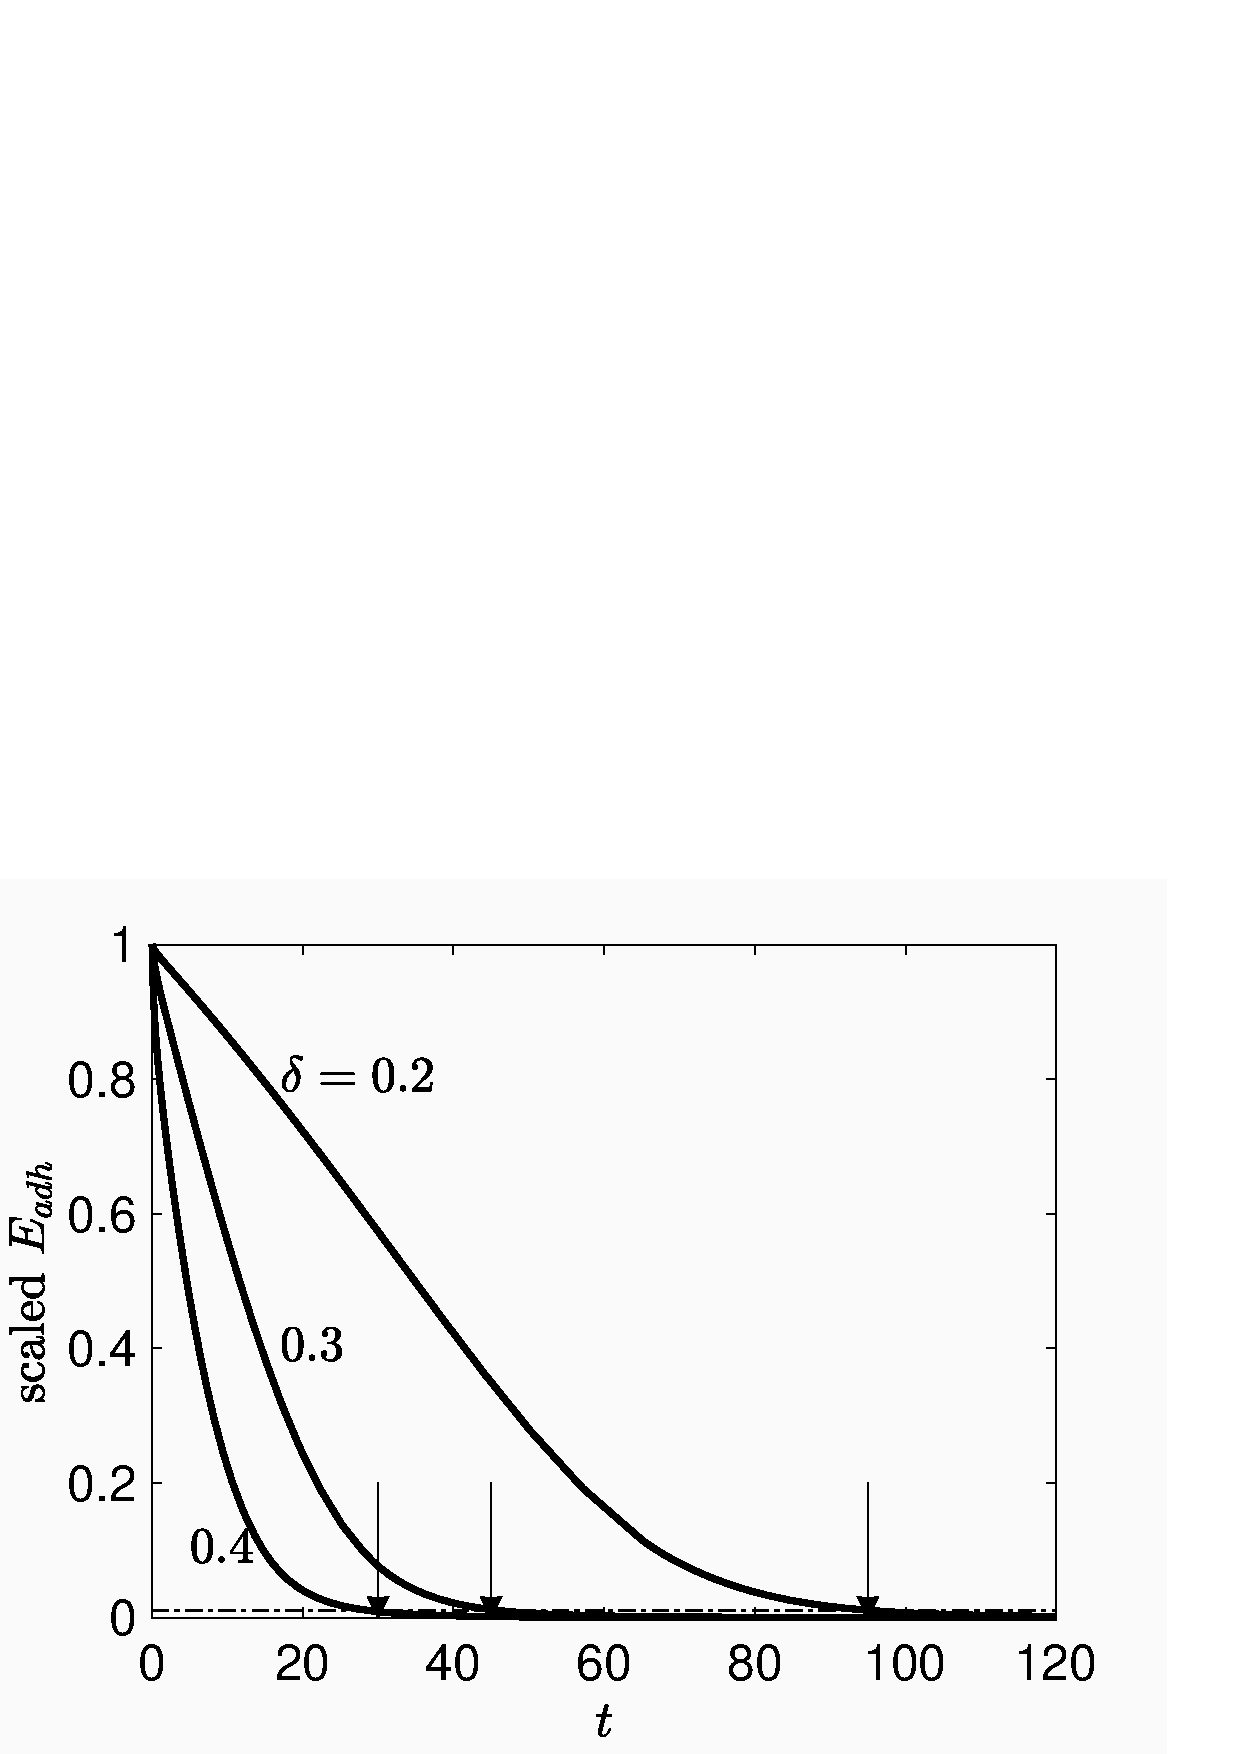
\includegraphics[keepaspectratio=true,scale=0.4]{figs/Dec13a_time_scaling01.png}
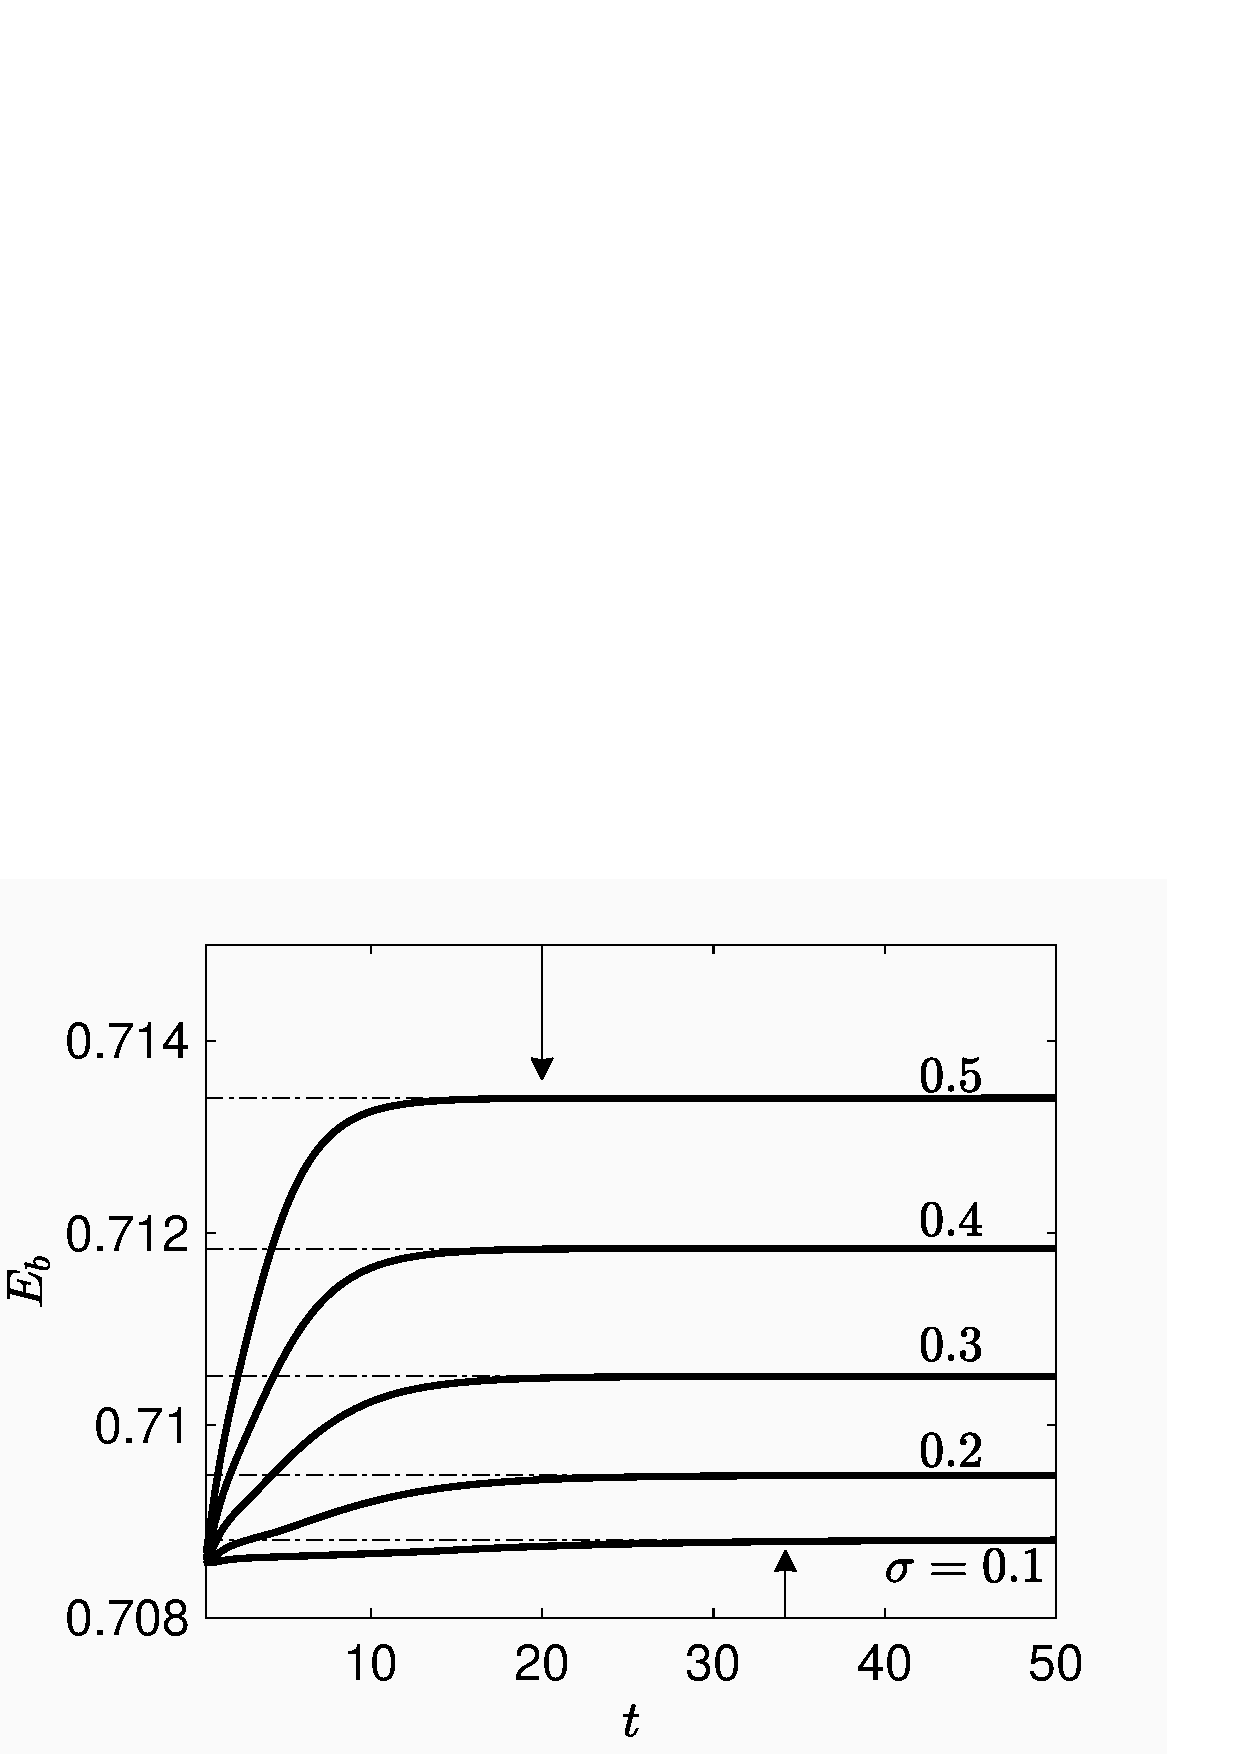
\includegraphics[keepaspectratio=true,scale=0.4]{figs/Dec13a_time_scaling02.png}
\caption{\label{fig:qflow00} Scaling of the time it takes for two
  vesicles to reach equilibrium. {\em Left}: Scaling with respect to
  $\delta$ with $\mathcal{H}=0.1$.  {\em Right}: Scaling with respect to
  $\mathcal{H}$ with
  $\delta = 0.4$. Arrows indicate the time by when the equilibrium is
  reached within $1\%$.}
\end{figure}

To test the scaling of the duration $t$ with respect to $\mathcal{H}$
and $\delta$, we simulate the vesicle adhesion dynamics in a quiescent
flow.  Starting with two vesicles at a distance of twice the vesicle
radius, the long-range attraction pulls the vesicles together.  The left
plot of Figure~\ref{fig:qflow00} shows the scaled adhesion energy versus
time with $\mathcal{H}=0.1$ and three values of $\delta$ as labeled.
Adhesion energy reaches minimum at equilibrium, and the scaled $E_{adh}$
evolves towards zero at equilibrium.  The arrows indicate the times when
the scaled adhesion energy reaches within $1\%$ of equilibrium: $t\sim
96$ for $\delta=0.2$, $t\sim 45$ for $\delta = 0.3$, and $t\sim 30$ for
$\delta=0.4$:
\begin{align*}
\frac{t_{\delta=0.2}}{t_{\delta=0.4}} \sim \frac{96}{30}=3.2 
  &\Longleftrightarrow \left(\frac{0.4}{0.2}\right)^{5/3}\sim 3.17,\\
\frac{t_{\delta=0.2}}{t_{\delta=0.3}} \sim \frac{96}{45}=2.1 
  &\Longleftrightarrow \left(\frac{0.3}{0.2}\right)^{5/3}\sim 2.
\end{align*}

The scaling with respect to adhesion strength $\mathcal{H}$ is
illustrated in the right plot of Figure~\ref{fig:qflow00}, where $\delta
= 0.4$ and $\mathcal{H}$ varies from $0.1$ to $0.5$ as labeled.  Again
the arrows indicate the times when the equilibrium is reached within
$1\%$:
\begin{align*}
  \frac{t_{\mathcal{H}=0.1}}{t_{\mathcal{H}=0.5}} \sim \frac{34}{20} = 1.71 
  &\Longleftrightarrow \left(\frac{0.5}{0.1}\right)^{1/3}\sim 1.71.
\end{align*}
From the above results, we conclude that the scaling in
equation~\eqref{eq:teq_scaling} captures the adhesion dynamics of two
vesicles that interact with each other via the adhesion force in
equation~\eqref{eq:Fh}.

%%%%%%%%%%%%%%%%%%%%%%%%%%%%%%%%%%%%%%%%%%%%%%%%%%%%%%%%%%%%%%%%%%%%%%%%
\subsection{Effects of the adhesion parameters on equilibrium
configuration of a vesicle pair}
\label{subsec:qflow_adhesion_parameters} We again simulate two identical
adhering vesicles with the adhesion force in equation~\eqref{eq:Fh}.
The initial vesicle separation is smaller than in the previous
simulations so that the equilibrium configuration is achieved in a
shorter time horizon.  Once a vesicle doublet is formed, the membrane
shape in the contact region depends on the adhesion strength relative to
the membrane bending rigidity.  For weak to moderate adhesion strength,
vesicle membranes are flattened in the contact region while the rest of
vesicle maintains a nearly spherical shape~\cite{EvansMetcalfe1984_BJ,
Book_PhysicalBasisCellAdhesion, Book_IntermolecularSurfaceForces,
RamachandranAndersonLealIsraelachvili2010_Langmuir}.  Under a strong
adhesion, however, the vesicle membranes in the contact region buckle
and form a sigmoidal shape that has also been observed in RBC
doublets~\cite{Ziherl2007_PRL, ZiherlSvetina2007_PNAS,
FlormannAouane2017_SciReports}.  An external electric field is also able
to buckle a vesicle membrane that is adhered to a solid
substrate~\cite{SteinkuhlerAgudo-Canalejo2016_BJ}.

%the vesicle may deform
%significantly in the contact region while still maintain nearly
%spherical shape on the opposite side to the contact
%region~\cite{EvansMetcalfe1984_BJ, Book_PhysicalBasisCellAdhesion, Book_IntermolecularSurfaceForces,RamachandranAndersonLealIsraelachvili2010_Langmuir}.
%In the contact region, vesicle membranes are flattened under a weak to moderate adhesive potential.
%Under a strong adhesion the vesicle membranes buckle and form a sigmoidal shape in the contact region \cite{Ziherl2007_PRL,ZiherlSvetina2007_PNAS,FlormannAouane2017_SciReports}.

In this work we focus on weakly adhesive vesicles whose equilibrium
shapes in a quiescent flow are shown in the left plot of
Figure~\ref{fig:Dec18_vesicle_shape} for three reduced areas: $\Delta
A=0.95$, $0.75$, and $0.6$ with $\mathcal{H}=5$ and $\delta = 0.2$. 
\begin{figure}
%  \includegraphics[keepaspectratio=true,scale=0.175]{figs/Dec18_vesicle_shape_vs_rA_00.jpeg}
%  \includegraphics[keepaspectratio=true,scale=0.175]{figs/Dec18_vesicle_shape_vs_rA_01.jpeg}
   \includegraphics[keepaspectratio=true,scale=0.5]{figs/Dec18_vesicle_shape_vs_rA_composite.png}
  \caption{\label{fig:Dec18_vesicle_shape} Equilibrium configurations of
  a doublet of identical vesicles under adhesion in a quiescent flow at
  three values of $\Delta A$.  The vesicle reduced areas of $\Delta
  A=0.95$, $0.75$, and $0.6$ are labeled.  The color coding is the
  tension along the vesicle.  The vesicle length is fixed at $2\pi$, the
  dimensionless bending rigidity modulus is $\kappa_b=1$, the Hamaker
  constant is $\mathcal{H}=5$, and the separation distance is
  $\delta=0.2$.  {\em Left}: The overall equilibrium shapes of two
  vesicles under adhesive interactions vary with the reduced area.  {\em
  Right}: The membrane shapes in the contact region.} 
\end{figure}
The equilibrium vesicle shape for $\Delta A=0.95$ is the circular cap
with a flat contact region.  This is similar to the observed shapes of
two vesicles under strong adhesive interaction
in~\cite{RamachandranAndersonLealIsraelachvili2010_Langmuir}.  When
vesicles are more deflated with a reduced area $\Delta A = 0.75$, the
equilibrium vesicle shape is elongated with a bigger contact region.
This is consistent with the equilibrium shapes of a vesicle doublet
under a $(m,n) = (12,6)$
L.-J.~potential~\cite{FlormannAouane2017_SciReports}.  As the reduced
area decreases further, we observe undulation of the vesicle membrane on
the non-contact side while the contact region remains flat.  The color
coding along each curve is the tension of the vesicle membrane.  We
observe that the membrane tension in the contact region is very
negative, indicating a dominant compression of membrane when the
adhesion force is strong to keep the vesicles bound together.

The right plot of Figure~\ref{fig:Dec18_vesicle_shape} is a zoom on the
membranes in the contact region, where the membranes are not perfectly
flat---at all reduced area we observe that the membranes are slightly
curved with a dip at the edge.  Such membrane undulation in the contact
region is predicted by lubrication analyses on a membrane under adhesion
with a solid substrate~\cite{BlountMiksisDavis2013_PRSa,
YoungStone2017_PRF}.  Also the dip at the edge of contact region is
related to but different from the buckling of membrane under strong
adhesion: A closer inspection on the dip at the edge shows that the
membrane distance is smaller than the neutral separation distance
$\delta$ there. Thus the adhesion force is attractive for most of the
membranes in the contact region except at the edge, where the adhesive
force turns repulsive.  Results from the lubrication analysis show that
this dip and slightly curved shape in the contact region are independent
of the adhesion strength. The high membrane curvature at the edge may
pose a problem for using the contact angle there to estimate the
adhesion strength. This inspires us to investigate the possibility of
using a dynamic fluid trap to measure the adhesion strength (see
Section~\ref{sec:eflow}).

\begin{figure}
\includegraphics[keepaspectratio=true,scale=0.175]{figs/Dec18_Ebleft_Eadhright_vs_rA_adR0p2_adS502.jpeg}
\includegraphics[keepaspectratio=true,scale=0.175]{figs/Dec18_EbEadh_vs_rA_adR0p2_adS502.jpeg}
  \caption{\label{fig:Dec18_vesicle_equilibrium1}   {\em Left}: The
  total bending energy (solid curve) and adhesion energy (dash-dotted
  curve) plotted against the reduced area $\Delta A$. {\em Right}: The
  sum of two energies plotted against reduced area $\Delta A$. The two
  vesicles in the doublet are of the same length and reduced area.  The
  Hamaker constant is $\mathcal{H} = 5$ and the separation distance is
  $\delta = 0.2$.}
\end{figure}

The left plot of Figure~\ref{fig:Dec18_vesicle_equilibrium1} shows the
total bending energy and adhesion energy as a function of the reduced
area. The smaller the reduced area, the more vesicle area is available
for deformation and thus the bending energy is higher.  In contrast, the
total adhesion energy becomes more negative as the reduced area
decreases.  The sum of two energies is plotted in the right plot of
Figure~\ref{fig:Dec18_vesicle_equilibrium1}, where a local minimum in
the total energy is found around $\Delta A = 0.85$.

\begin{figure}
\includegraphics[keepaspectratio=true,scale=0.18]{figs/Dec18_Eb_vs_sigma_rA0p9502.jpeg}
\includegraphics[keepaspectratio=true,scale=0.18]{figs/Dec18_Eadh_vs_sigma_rA0p9502.jpeg}
  \caption{\label{fig:Dec18_equilibrium} 
  The total bending energy ({\em left}) and adhesion energy ({\em
  right}) of a vesicle doublet at equilibrium versus the adhesion
  strength $\mathcal{H}$.  The two identical vesicles in the doublet
  have a length of $2\pi$ and a reduced area of $\Delta A=0.95$, with
  separation distance $\delta = 0.2$ (triangles), $0.3$ (crosses), and
  $0.4$ (circles).}
\end{figure}

Figure~\ref{fig:Dec18_equilibrium} demonstrates how the adhesion
strength $\mathcal{H}$ and separation distance $\delta$ affect the
equilibrium configuration of two vesicles under adhesive interactions.
Both vesicles have a length of $2\pi$ and a reduced area of $\Delta A =
0.95$.  The total bending (left) and adhesion (right) energies at
equilibrium are plotted against $\mathcal{H}$ for three values of the
separation distance $\delta$.  We observe that for $\Delta A=0.95$ the
equilibrium vesicle shape does not vary much with the adhesion strength
$\mathcal{H}$, while the total adhesion energy varies linearly with
$\mathcal{H}$.

%% \begin{figure}
%% 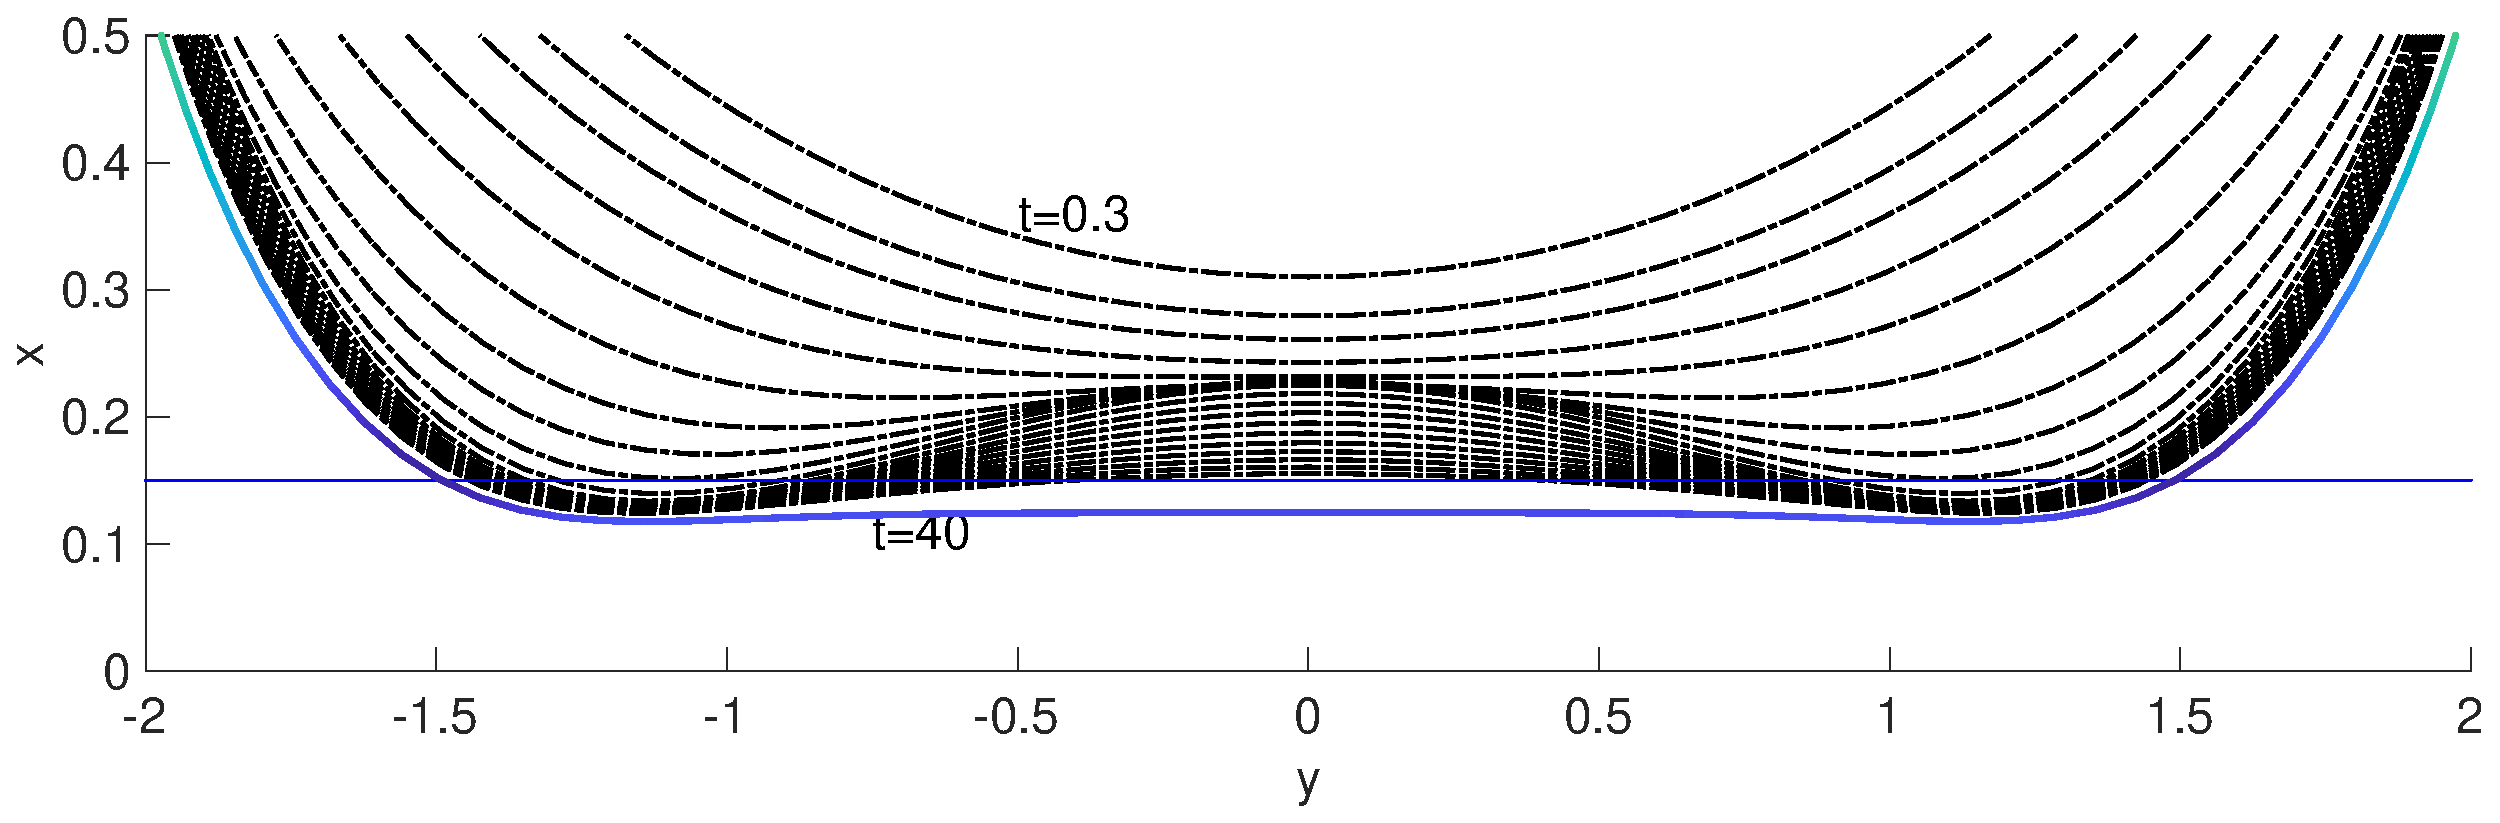
\includegraphics[keepaspectratio=true,scale=0.4]{figs/relax2Ves01g-draining01a.eps}
%% \caption{Adhesion dynamics of two vesicles with $\delta = 0.3$. From $t=0.3$ to $t=40$, the time interval $\delta t = 0.3$ between every two neighboring dash-dotted curves.}
%% \label{fig:qflow_g-draining01a}
%% \end{figure}
%
%% \begin{figure}
%% 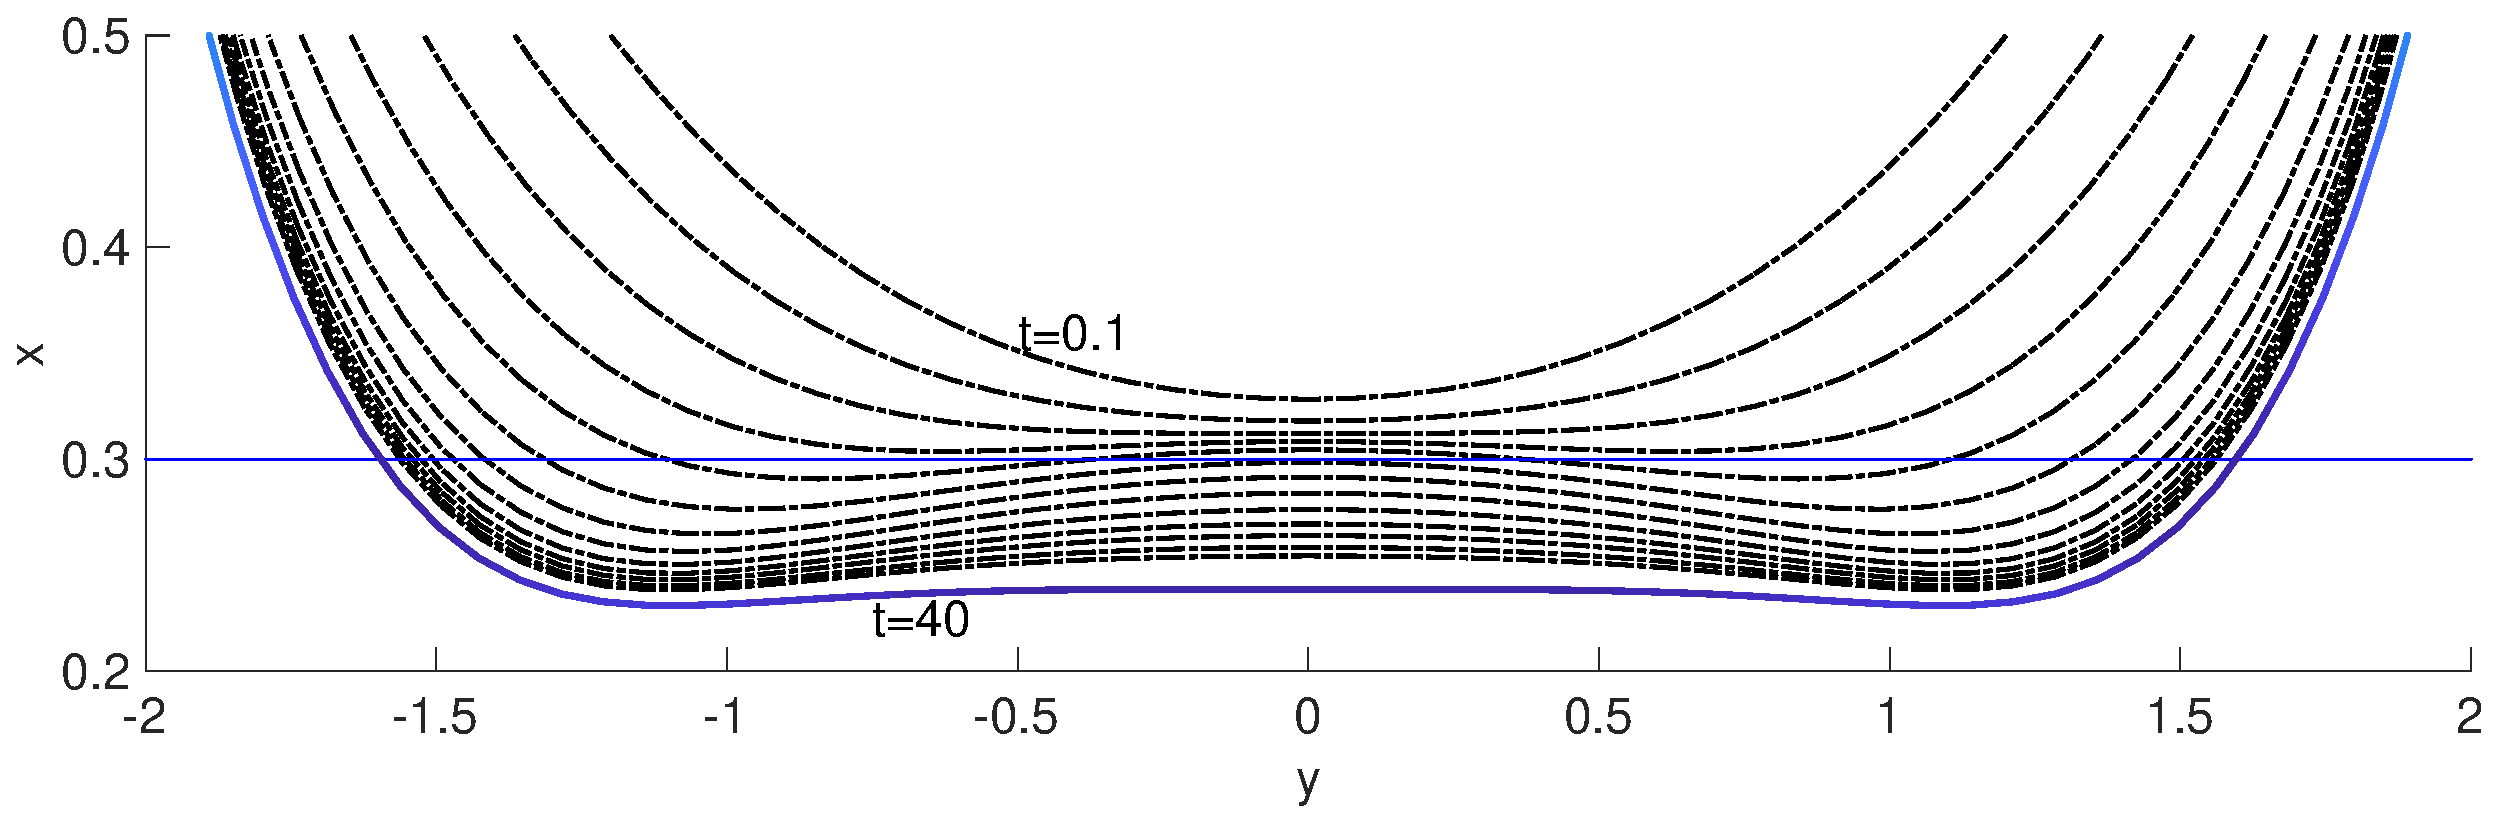
\includegraphics[keepaspectratio=true,scale=0.4]{figs/relax2Ves01j-draining01a.eps}
%% \caption{Adhesion dynamics of two vesicles with $\delta = 0.6$. From $t=0.1$ to $t=40$, the time interval $\delta t = 0.1$ between every two neighboring dash-dotted curves.}
%% \label{fig:qflow_g-draining01a}
%% \end{figure}
%
%%%%%%%%%%%%%%%%%%%%%%%%%%%%%%%%%%%%%%%%%%%%%%%%%%%%%%%%%%%%%%%%%%%%%%%%%
%\subsection{Effects of reduced area}
%\label{sec:qflow_reduced_area} 
%Figure~\ref{fig:qflow_reduced_area}
%
%\begin{figure}
%\includegraphics[keepaspectratio=true,scale=0.5]{figs/nrelax2Ves02o_rA.png}
%\caption{The effect of the reduced area on adhering vesicles in a
%quiescent flow.  The parameters of the vdW potential are $\delta = 0.2$
%and $\sigma = 0.5$.}
%\label{fig:qflow_reduced_area}
%\end{figure}
%
%% \begin{figure}
%% 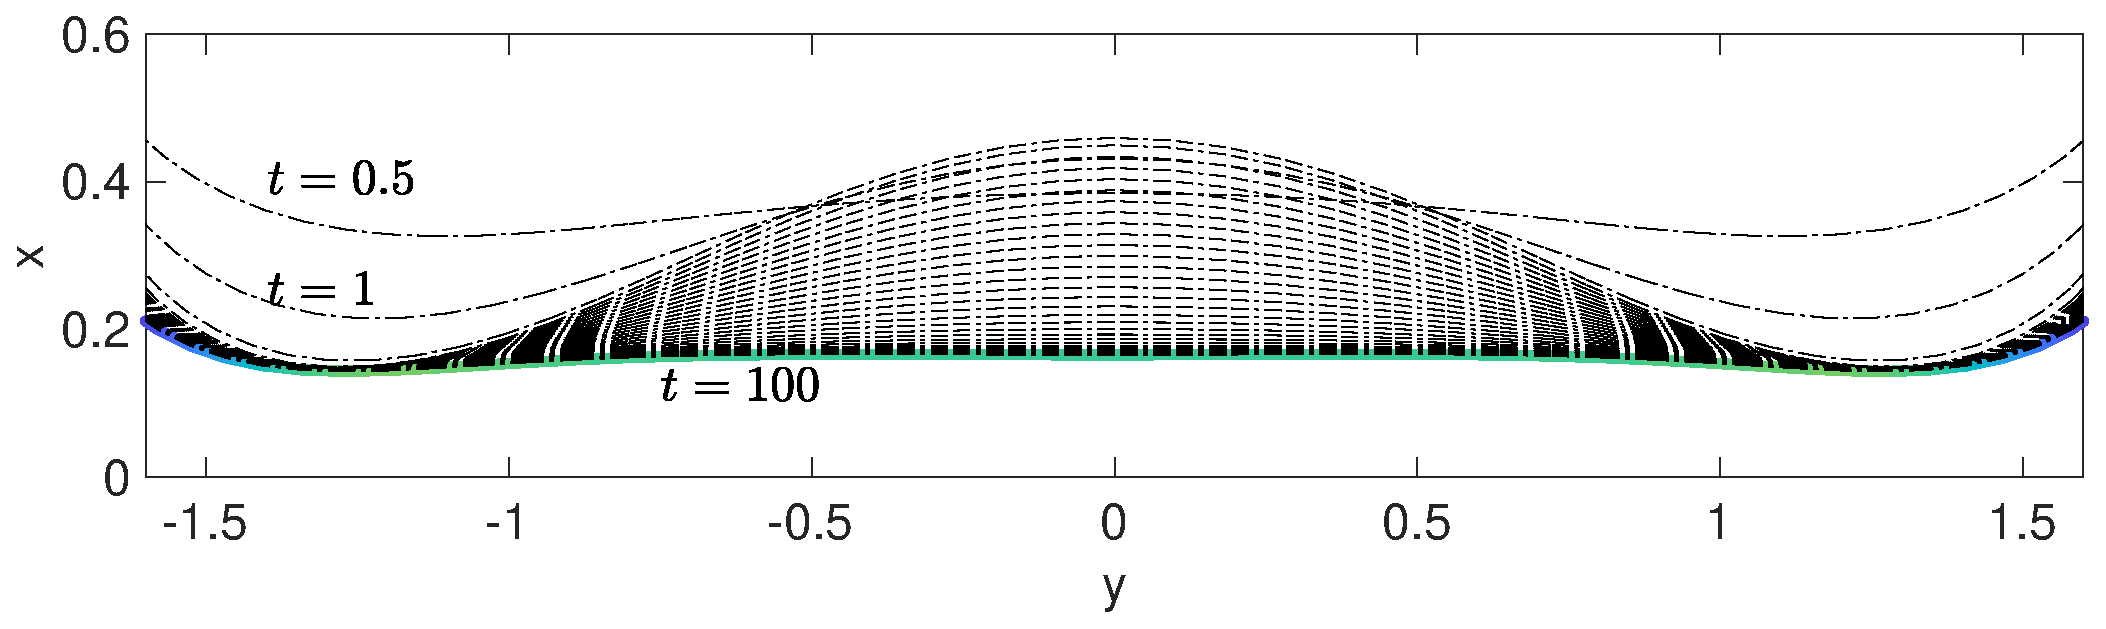
\includegraphics[keepaspectratio=true,scale=0.4]{figs/relax2Ves01usa.eps}
%% \caption{Adhesion dynamics of two vesicles with $\delta = 0.4$ and $\sigma=0.2$. From $t=0.06$ to $t=100$, the time interval $\delta t = 0.06$ between every two neighboring dash-dotted curves.}
%% \label{fig:qflow_u-draining}
%% \end{figure}
%
%% \begin{figure}
%% 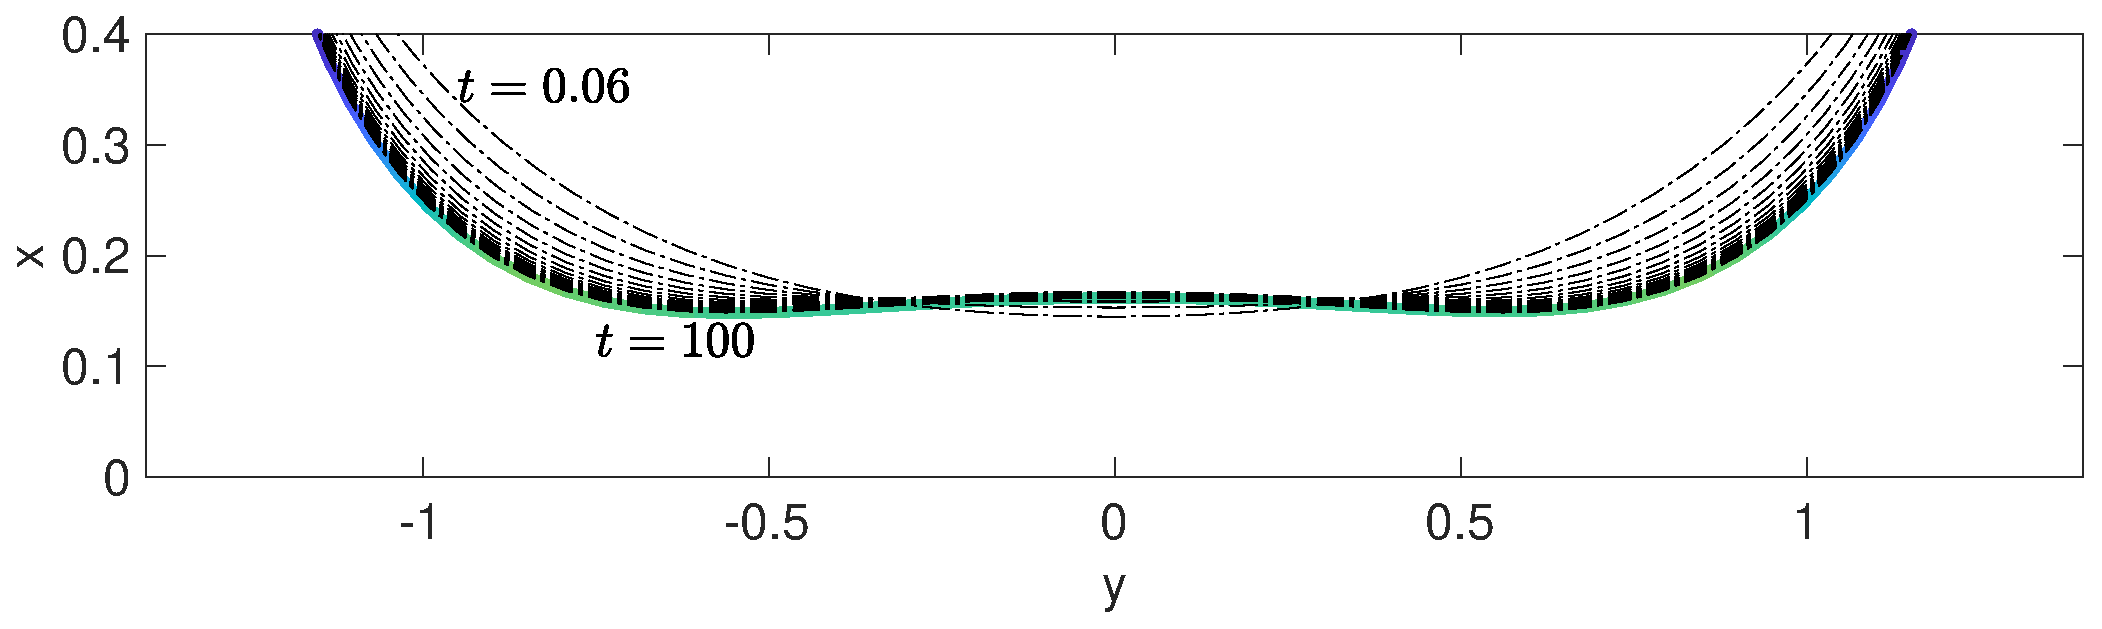
\includegraphics[keepaspectratio=true,scale=0.4]{figs/relax2Ves01zsa.eps}
%% \caption{Adhesion dynamics of two vesicles with $\delta = 0.4$ and $\sigma=0.2$. From $t=1$ to $t=100$, the time interval $\delta t = 1$ 
%% between every two neighboring dash-dotted curves.}
%% \label{fig:qflow_z-draining}
%% \end{figure}

%%%%%%%%%%%%%%%%%%%%%%%%%%%%%%%%%%%%%%%%%%%%%%%%%%%%%%%%%%%%%%%%%%%%%%%%
\section{Adhesion of two vesicles in an extensional flow} 
\label{sec:eflow} 
The hydrodynamics of a single vesicle in an extensional flow has
revealed novel nonlinear vesicle dynamics not found for a viscous
drop~\cite{KantslerSegreSteinberg2008_PRL, ZhaoShaqfeh2013_JFM,
Narsimhan2014_JFM, DahlNarsimhanGouveia2016_SoftMatt}.  The stagnation
point (zero-velocity at the origin) in an extensional flow, $\uu
=\chi(-x,y)$, is a saddle point where two laminar streams converge along
an axis and then diverge in the orthogonal direction.  With an active
control algorithm to place the stagnation point at a desirable location
by adjusting the streaming flow strength with a feedback
loop~\cite{Johnson-Chavarria2011_EMJ}, a particle can be trapped at the
stagnation point for long time scales to facilitate image acquisition or
other detailed measures such as particle image velocimetry of flow
inside and around the particle.  To explore the application of such a
fluid trap to measure the adhesion strength between two bound vesicle
membranes, we propose the following thought experiment.  Beginning with
two identical vesicles in an equilibrium configuration that form a
doublet with a flat contact region
(Figure~\ref{fig:Dec18_vesicle_shape}), we turn on the fluid trap with
the stagnation point placed at the center of the vesicle doublet.
Depending on the Hamaker constant, we expect that either the flow
overcomes the adhesive force and the doublet is broken, or the adhesive
force is sufficiently strong and the doublet reaches a stable stationary
configuration.

In the following numerical experiments we initially place a vesicle
doublet with $\theta=\pi$, so that the diverging flow may be strong
enough to pull vesicles away from the doublet.  At low extensional
rates, we expect the doublet to stay bound at the fluid trap stagnation
point.  On the other hand, the vesicle doublet may become unstable and
eventually separate at higher extensional rates.  Thus we expect there
to exist a critical extensional rate $\chi_c$ above which the vesicle
doublet cannot stay bound under a given adhesion potential.  Therefore,
the dependence of the critical extensional rate $\chi_c$ on the adhesion
potential and the mechanical vesicle properties provides a means to
probe the physics of membrane adhesion.

\begin{figure}[htp]
   \includegraphics[width=0.25\textwidth]{figs/rotate1.pdf}
   \hspace{20pt}
   \includegraphics[width=0.25\textwidth]{figs/angleDefinition.pdf}
   \hspace{20pt}
   \includegraphics[width=0.25\textwidth]{figs/rotate2.pdf}
   \caption{\label{fig:InclinationAngle} The definition of the
   inclination angle of a vesicle doublet at the center of an
   extensional flow.  An inclination angle of $\pi$ indicates a doublet
   whose long axis is orthogonal to the diverging direction, while an
   inclination angle of $\pi/2$ indicates a doublet whose short axis is
   orthogonal to the diverging direction.  The square mark is a
   stagnation point and the round point is located at the center of the
   vesicle.  The initial configurations in this section all have an
   inclination angle of $\theta = \pi$.}
 \end{figure}

Based on how the contact region aligns with the extensional flow, we can
define the inclination angle of the vesicle doublet as illustrated in
Figure~\ref{fig:InclinationAngle}. When $\theta=\pi$, the doublet long
axis is aligned with the far-field converging flow, and the diverging flow
pulls the vesicles apart from each other and the long-range attractive
force is essential to keep the two vesicles from separating.  In
contrast, when $\theta = \pi/2$, the doublet long axis is aligned with
the diverging flow, the converging flow pushes the vesicles towards
each other and the short-range repulsive force is essential to keep the
two vesicles at the separation distance.  With the converging flow
pushing the two vesicles towards the stagnation point dynamically placed
at the doublet center, this configuration is expected to be more stable
than the $\theta=\pi$ configuration in the left of
Figure~\ref{fig:InclinationAngle}. This is because when $\theta=\pi$ the
diverging flow is pulling the vesicles away from each other as shown in
the illustration.  However, when the doublet inclination angle is fixed
at $\theta=\pi/2$, the vesicle doublet stays intact if the adhesive
force is strong enough to dominate the fluid drag.  However, it is
possible that the diverging flow may overcome adhesion and break up the
doublet.  It is also reasonable to expect a vesicle doublet to rotate
from the less stable configuration $\theta=\pi$ to the more stable
configuration $\theta=\pi/2$, so that the fluid flow is pushing them
together rather than pulling them apart.

We consider vesicle doublets with reduced areas 0.70, 0.75, 0.80, 0.85,
0.90, and 0.95, all with a length of $2\pi$, and we vary the extensional
rate, $\chi$, between $10^{-2}$ and $10^{-1}$.  Since the stagnation
point can be controlled in an experimental
setting~\cite{Johnson-Chavarria2011_EMJ}, we mimic the active control of
the microfluidic experiments by moving the center of the doublet at each
time step so that the stagnation point occurs exactly in the middle of
the doublet.  With this adjustment, the vesicles either remain as a
doublet in the fluid trap centered around the stagnation point, or the
doublet is broken and the vesicles separate from one another.  In
Figures~\ref{fig:extensional1}, snapshots of a fluid trap containing a
vesicle doublet of reduced area $\Delta A = 0.7$ are simulated at three
different extensional rates.  We observe that the doublet rotates from
$\theta=\pi$ configuration towards the more stable $\theta=\pi/2$
configuration, as shown in Figures~\ref{fig:extensional1}.  We also
observe that with moderate extensional rates, the doublet falls short of
aligning their long axis with the diverging direction.  Moreover, the
final inclination angle is closest to the stable $\theta=\pi/2$ for the
smallest extensional rates.  While this doublet remains bound for all
the considered extensional rates, a doublet with a reduced area of
$\Delta A = 0.8$ is split with a critical extensional rate $\chi_c =
0.1$ (Figure~\ref{fig:extensional3}).  

\begin{figure}[htp]
  \includegraphics[width = 0.16\textwidth,trim={4cm 2cm 4cm 1cm},clip]{figs/extensional_adR4em1adS7em1Chi2em2_ra070_image01.png}
  \includegraphics[width = 0.16\textwidth,trim={4cm 2cm 4cm 1cm},clip]{figs/extensional_adR4em1adS7em1Chi2em2_ra070_image02.png}
  \includegraphics[width = 0.16\textwidth,trim={4cm 2cm 4cm 1cm},clip]{figs/extensional_adR4em1adS7em1Chi2em2_ra070_image03.png}
  \includegraphics[width = 0.16\textwidth,trim={4cm 2cm 4cm 1cm},clip]{figs/extensional_adR4em1adS7em1Chi2em2_ra070_image04.png}
  \includegraphics[width = 0.16\textwidth,trim={4cm 2cm 4cm 1cm},clip]{figs/extensional_adR4em1adS7em1Chi2em2_ra070_image05.png}\\
   \includegraphics[width = 0.16\textwidth,trim={4cm 2cm 4cm 1cm},clip]{figs/extensional_adR4em1adS7em1Chi7em2_ra070_image01.png}
  \includegraphics[width = 0.16\textwidth,trim={4cm 2cm 4cm 1cm},clip]{figs/extensional_adR4em1adS7em1Chi7em2_ra070_image02.png}
  \includegraphics[width = 0.16\textwidth,trim={4cm 2cm 4cm 1cm},clip]{figs/extensional_adR4em1adS7em1Chi7em2_ra070_image03.png}
  \includegraphics[width = 0.16\textwidth,trim={4cm 2cm 4cm 1cm},clip]{figs/extensional_adR4em1adS7em1Chi7em2_ra070_image04.png}
  \includegraphics[width = 0.16\textwidth,trim={4cm 2cm 4cm 1cm},clip]{figs/extensional_adR4em1adS7em1Chi7em2_ra070_image05.png} \\
  \includegraphics[width = 0.16\textwidth,trim={4cm 2cm 4cm 1cm},clip]{figs/extensional_adR4em1adS7em1Chi1em1_ra070_image01.png}
  \includegraphics[width = 0.16\textwidth,trim={4cm 2cm 4cm 1cm},clip]{figs/extensional_adR4em1adS7em1Chi1em1_ra070_image02.png}
  \includegraphics[width = 0.16\textwidth,trim={4cm 2cm 4cm 1cm},clip]{figs/extensional_adR4em1adS7em1Chi1em1_ra070_image03.png}
  \includegraphics[width = 0.16\textwidth,trim={4cm 2cm 4cm 1cm},clip]{figs/extensional_adR4em1adS7em1Chi1em1_ra070_image04.png}
  \includegraphics[width = 0.16\textwidth,trim={4cm 2cm 4cm 1cm},clip]{figs/extensional_adR4em1adS7em1Chi1em1_ra070_image05.png}
  \caption{\label{fig:extensional1} A vesicle doublet in an extensional
  flow with an initial inclination angle $\theta=\pi$.  The reduced
  area is $\Delta A = 0.7$, the Hamaker constant is $\mathcal{H} = 0.7$,
  the separation distance is $\delta = 0.4$, and the extensional rate is
  $\chi = 0.02$ ({\em top}), $\chi=0.07$ ({\em middle}), and $\chi =
  0.1$ ({\em bottom}).  The center of the vesicle, denoted with a black
  square, is the stagnation point.}
  \end{figure}

 \begin{figure}
    \includegraphics[width = 0.16\textwidth,trim={4cm 2cm 4cm 1cm},clip]{figs/extensional_adR4em1adS7em1Chi1em1_ra080_image01.png}
  \includegraphics[width = 0.16\textwidth,trim={4cm 2cm 4cm 1cm},clip]{figs/extensional_adR4em1adS7em1Chi1em1_ra080_image02.png}
  \includegraphics[width = 0.16\textwidth,trim={4cm 2cm 4cm 1cm},clip]{figs/extensional_adR4em1adS7em1Chi1em1_ra080_image03.png}
  \includegraphics[width = 0.16\textwidth,trim={4cm 2cm 4cm 1cm},clip]{figs/extensional_adR4em1adS7em1Chi1em1_ra080_image04.png}
  \includegraphics[width = 0.16\textwidth,trim={4cm 2cm 4cm 1cm},clip]{figs/extensional_adR4em1adS7em1Chi1em1_ra080_image05.png}
  \caption{\label{fig:extensional3} A vesicle doublet in an extensional
  flow with an initial inclination angle $\theta=\pi$.  The reduced area
  is $\Delta A = 0.8$, the Hamaker constant $\mathcal{H} = 0.7$, the
  separation distance is $\delta = 0.4$, and the extensional rate $\chi
  = 0.1$.  The center of the vesicle, denoted with a black square, is a
  stagnation point.}
\end{figure}

In Figure~\ref{fig:extensionalInclinationAngle}, we plot the inclination
angle of the doublet as a function of time for four different
extensional rates (left) and the final inclination angle for all
doublets that reach an equilibrium state (middle).  We observe that not
only do smaller extensional rates result in smaller inclination
angles, but smaller reduced areas also result in smaller inclination
angles.  
%
%From physics we expect that stronger adhesion is required to keep 
%the vesicle doublet intact under a fluid trap as we increase the flow rate.
%
%It is less obvious how the critical adhesion strength depends on the reduced area of the vesicles.
%
%Even though we only used one value of Hamaker constant (${\cal H} = 0.7$) we expect that
%
%Moreover, the critical Hamaker constant that determines if the
%doublet remains trapped or is broken decreases with an increasing
%extensional rate \todo[inline]{not sure how we can say this since we've
%only considered one Hamaker constant}.  
%
We summarize the final
inclination angle of the doublet in the right plot of
Figure~\ref{fig:extensionalInclinationAngle}.  
The size of the round
dots are scaled to the final inclination angle as defined in
Figure~\ref{fig:InclinationAngle}.  At smaller extensional rates, the
vesicles come closer to aligning their long axis with the diverging
direction.  When the doublet is broken at reduced area $\Delta A =
0.80$, the extensional rate is sufficiently large to align the long axis
of the vesicle with the diverging direction and then the vesicles
separate (Figure~\ref{fig:extensional3}).  For very low extensional
rates, the time horizon is insufficient for the doublet to reach an
equilibrium state, and these simulations are marked with a square.  The
right plot of Figure~\ref{fig:extensionalInclinationAngle} also
summarizes the reduced areas and extensional rates that result in a
bound vesicle doublet in a fluid trap: Parameter values with a blue mark
result in a fluid trap and parameter values with a red mark result in
vesicle separation.

\begin{figure}[htp]
  \includegraphics[height=0.27\textwidth]{figs/adR4em1adS7em1_ra070_inclinationAngle.pdf}
  \includegraphics[height=0.27\textwidth]{figs/adR4em1adS7em1_finalInclinationAngle.pdf}
  \includegraphics[height=0.27\textwidth]{figs/extensional_adR4em1adS7em1_phaseDiagram.pdf}
  \caption{\label{fig:extensionalInclinationAngle} {\em Left}: The
  inclination angle of a doublet formed by vesicles of reduced area
  $\Delta A = 0.7$ in an extensional flow with an extensional rate
  $\chi$.  {\em Middle}: The final inclination angle of doublets.  At
  larger extensional rates, the doublet is broken by the flow.  {\em
  Right}: A phase diagram of the long-time behavior of a fluid trap
  formed by two adhering vesicles in an extensional flow.  Results are
  not reported for some of the low extensional rates since the doublet
  had not tilted to an equilibrium inclination angle for the given time
  horizon.}
\end{figure}

Finally, to further characterize the rotating dynamics of a doublet in
the fluid trap, we compute and plot the vorticity and total force on a
doublet with identical vesicles with reduced area $\Delta A=0.7$,
Hamaker constant $\mathcal{H} = 0.7$, separation distance $\delta =
0.4$, and extensional rate $\chi = 0.7$ in
Figure~\ref{fig:extensionalVorticity}.  Starting from a vesicle doublet
with an initial inclination angle $\theta=\pi$, the doublet slowly
begins to rotate around $t\sim 250$.  We notice that the net force on
each vesicle is almost anti-parallel to the diverging flow in the
far-field so to balance the hydrodynamic drag force that pulls the
vesicles apart.  Then, as the doublet starts to rotate, each vesicle
experiences a drag force from both the up and down diverging streaming
flows.  For small extensional rate, the rotation will continue until
$\theta = \pi/2$ so the doublet remains perfectly symmetric with respect
to their mid-plane and each vesicle experiences drag forces that cancel
in both directions.  For slightly higher extensional rate, we observe
that the two vesicles slide against each other as the doublet rotates.
The slight sliding motion leads to a transition in the contact region
membrane shape from a bulging profile to an S-shape profile of nearly
uniform height except near the edge of contact region.  This adjustment
greatly reduces the net force on each vesicle, leading to an equilibrium
configuration with an inclination angle $\theta > \pi/2$ as shown in the
left of Figure~\ref{fig:extensionalInclinationAngle}.  Finally, the
vorticity and the flow between the vesicles approaches zero and the
result is a fluid trap containing the doublet.
\begin{figure}[htp]
  \includegraphics[height = 0.26\textwidth,trim={6cm 1cm 5cm
  0cm},clip]{figs/extensionalVorticity01.png}
  \includegraphics[height = 0.26\textwidth,trim={6cm 1cm 5cm
  0cm},clip]{figs/extensionalVorticity02.png}
  \includegraphics[height = 0.26\textwidth,trim={6cm 1cm 5cm
  0cm},clip]{figs/extensionalVorticity03.png}
  \includegraphics[height = 0.26\textwidth,trim={6cm 1cm 5cm
  0cm},clip]{figs/extensionalVorticity04.png}
  \includegraphics[height = 0.26\textwidth,trim={5cm 1cm 2cm
  0cm},clip]{figs/extensionalVorticity05.png} \\
  \includegraphics[height = 0.26\textwidth,trim={6cm 1cm 5cm
  0cm},clip]{figs/extensionalVorticity06.png}
  \includegraphics[height = 0.26\textwidth,trim={6cm 1cm 5cm
  0cm},clip]{figs/extensionalVorticity07.png}
  \includegraphics[height = 0.26\textwidth,trim={6cm 1cm 5cm
  0cm},clip]{figs/extensionalVorticity08.png}
  \includegraphics[height = 0.26\textwidth,trim={6cm 1cm 5cm
  0cm},clip]{figs/extensionalVorticity09.png}
  \includegraphics[height = 0.26\textwidth,trim={5cm 1cm 2cm
  0cm},clip]{figs/extensionalVorticity10.png}
  \caption{\label{fig:extensionalVorticity} The vorticity and total
  force of two vesicles in a doublet.  The reduced area is $\Delta A =
  0.7$, the separation distance is $\delta = 0.4$, the Hamaker constant
  is $\mathcal{H} = 0.7$, and the extensional rate is $\chi = 0.7$.}
\end{figure}


%%%%%%%%%%%%%%%%%%%%%%%%%%%%%%%%%%%%%%%%%%%%%%%%%%%%%%%%%%%%%%%%%%%%%%%%
\section{Adhesion of two vesicles in a shear flow}
\label{sec:sflow} 
We consider two vesicles suspended in the shear flow $\uu = \chi(y,0)$,
where $\chi$ is the shear rate.  The vesicles are placed on the $y$ axis
so that the background velocity drives the vesicles towards one another.
In the absence of adhesion, once the vesicles are sufficiently close,
they are deflected to opposite sides of the $y$ axis, pass one another,
and separate from one another.  However, in the presence of adhesion,
the vesicles can form a doublet for certain values of the adhesion
length scale $\delta$, Hamaker constant $\mathcal{H}$, shear rate
$\chi$, and reduced area $\Delta A$.  Figure~\ref{fig:doublet090} shows
snapshots two vesicles that have formed a doublet and the color coding
is the tension along the vesicle.  The two vesicles are
identical with reduced area is $\Delta A = 0.9$, the shear rate is $\chi
= 0.5$, the adhesion length scale is $\delta = 0.4$, and the Hamaker
constant is $\mathcal{H} = 0.7$.  Similar to the quiescent example, we
observe that the membrane tension in the contact region is negative in
the contact region indicating that the membrane is being compressed when
the adhesive force is strongest.  Once the vesicles have formed a
doublet, the vesicles rotate in tandem rather than performing the usual
tank-treading motion.

\begin{figure}[htp]
  \includegraphics[width=0.24\textwidth]{figs/adR4em1adS7em1Chi5em1_ra090_image01.png}
  \includegraphics[width=0.24\textwidth]{figs/adR4em1adS7em1Chi5em1_ra090_image02.png}
  \includegraphics[width=0.24\textwidth]{figs/adR4em1adS7em1Chi5em1_ra090_image03.png}
  \includegraphics[width=0.24\textwidth]{figs/adR4em1adS7em1Chi5em1_ra090_image04.png}
  \includegraphics[width=0.24\textwidth]{figs/adR4em1adS7em1Chi5em1_ra090_image05.png}
  \includegraphics[width=0.24\textwidth]{figs/adR4em1adS7em1Chi5em1_ra090_image06.png}
  \includegraphics[width=0.24\textwidth]{figs/adR4em1adS7em1Chi5em1_ra090_image07.png}
  \includegraphics[width=0.24\textwidth]{figs/adR4em1adS7em1Chi5em1_ra090_image08.png}
  \caption{\label{fig:doublet090} The formation of a doublet in a shear
  flow.  The reduced area is $\Delta A = 0.9$, the Hamaker constant is
  $\mathcal{H}=0.7$, the adhesion length scale is $\delta = 0.4$, and
  the shear rate is $\chi=0.5$.}
\end{figure}

We characterize the effect of the Hamaker constant and shear rate by
determining a critical Hamaker constant, $\mathcal{H}_c$, which
determines if the vesicles form a doublet or separate.  We fix the
adhesion length scale to $\delta = 0.4$ and the vesicle reduced area to
$\Delta A = 0.9$.  In the left plot of
Figure~\ref{fig:sflow_phase_diagram}, we plot the minimum distance
between the vesicles as a function of time for various Hamaker
constants.  The red curves correspond to Hamaker constants that are too
small to bind the vesicles into a doublet, and the blue curves
correspond to Hamaker constants that are sufficiently large to form a
doublet.

\begin{figure}
  \includegraphics[height=0.35\textwidth]{figs/shear_adR4em1Chi1e0_ra-090.pdf}
  \includegraphics[height=0.35\textwidth]{figs/shear_adR4em1_ra090_phaseDiagram.pdf}
  \caption{{\em Left}: Distance between a pair of vesicles in a planar
  shear flow with shear rate $\chi=0.5$ and adhesion length scale
  $\delta = 0.4$.   The different lines correspond to a linear spacing
  of adhesion strengths ranging from $\mathcal{H}=0.1$ and
  $\mathcal{H}=1.0$.  {\em Right}: Phase diagram of vesicle
  hydrodynamics in a shear flow.  At a fixed reduced area $\Delta
  A=0.90$ and $\delta = 0.4$,  the critical Hamaker constant
  $\mathcal{H}$ for binding of two vesicles in a shear flow depends on
  the shear rate $\chi$.
\label{fig:sflow_phase_diagram}}
\end{figure}

Finally, we investigate the rheology of a suspension of a doublet by
computing the effective viscosity of a doublet and compare it to the
effective viscosity of a single tank-treading vesicle. The effective
viscosity is defined as the viscosity of a homogeneous Newtonian fluid
with the same energy dissipation per macroscopic element of fluid.  In a
simple shear flow, the intrinsic viscosity, $[\mu]$ is
\begin{align*}
  [\mu]:= \frac{\mu_{\mathrm{eff}} - \mu_0}{\phi \mu_0} = 
  \frac{1}{\chi \mu_0 T} \int_{T_i}^{T_e} 
  \langle \sigma_{12} \rangle dt,
\end{align*}
where
\begin{align*}
  \langle \tau \rangle = \frac{1}{|\omega|} \int_{\gamma}
    \xxi \otimes \xx ds,
\end{align*}
where $\phi$ is the area fraction of vesicles, $\tau$ is the stress due
to the vesicles, and $\langle \cdot \rangle$ is the spatial average.

In the left plot of Figure~\ref{fig:shearIntrinsicViscosity}, we compare
the intrinsic viscosity of a single tank-treading vesicle to a doublet.
To validate our simulations, we superimpose (black marks) the intrinsic
viscosity calculated by Ghigliotti {\em et
al.}~\cite{GhigliottiBibenMisbah2010_JFM}.  The presence of the doublet
significantly increases the intrinsic viscosity at all the reduced
areas.  To further characterize the effect of adhesion, in the right
plot of Figure~\ref{fig:shearIntrinsicViscosity} we decompose the
intrinsic viscosity into the contributions from the bending and tension
(blue), and the contribution from the adhesion (red).  We also
superimpose twice the intrinsic viscosity of a single tank-treading
vesicle (dashed curve) to demonstrate that the bending and tension of
the doublet behave similarly, but not identically, to a dilute
suspensions of non-adhering tank-treading vesicles.  We see that the
effect of the adhesion on the intrinsic viscosity is largest for
vesicles with small reduced areas.

\begin{figure}[htp]
  \centering
  \includegraphics[width=0.45\textwidth]{figs/shear2Ves_adR4em1adS7em1Chi5em1.pdf}
  \includegraphics[width=0.45\textwidth]{figs/doublet_decomp.pdf}
  \caption{\label{fig:shearIntrinsicViscosity} {\em Left}: The intrinsic
  viscosity of a tank-treading vesicle (blue) and a doublet (red).  The
  shear rate is $\chi = 0.5$, the Hamaker constant is $\mathcal{H} =
  0.7$, and the adhesion length scale is $\delta = 0.4$, and the length
  of the vesicles are held fixed.  The black marks denote intrinsic
  viscosity values computed by Ghigliotti {\em et
  al.}~\cite{GhigliottiBibenMisbah2010_JFM} (cf.~Figure 5).  {\em
  Right}: The decomposition of the intrinsic viscosity into the
  contributions for the bending and tension (blue) of the vesicles, and
  the contribution from the vesicle adhesion (red).  Also included is
  twice the intrinsic viscosity of a single tank-treading vesicle
  (dashed black line).}
\end{figure}



%%%%%%%%%%%%%%%%%%%%%%%%%%%%%%%%%%%%%%%%%%%%%%%%%%%%%%%%%%%%%%%%%%%%%%%%
\section{Conclusions\label{sec:conclusions}}
In this work we use boundary integral formulation with adaptive
time-stepping to simulate hydrodynamics of two vesicles with adhesive
interactions.  In a quiescent flow, two vesicles that are initially
sufficiently far apart move towards each other under a long-range
attraction.  We use a lubrication theory to estimate the time required
to reach the separation distance $\delta$, and the theoretical scaling is in good
agreement with numerical results.  Once two membranes are within
separation distance $\delta$, the adhesive force turns repulsive and the
membranes flatten to form a contact region.  Our simulations show that
the membranes in the contact region are actually curved with end points
at the shortest distance.  Once a vesicle doublet forms, we examine the
dependence of membrane bending and adhesion energies on the reduced
area, the Hamaker constant, and the separation distance.

Next we conduct a numerical experiment where a vesicle doublet is placed
at the center of a fluid trap, which can be actively controlled in
microfluidic channel so that fluid trap center is effectively the
stagnation point of an extensional flow characterized by a extensional
flow rate.  At low flow rate, we find the doublet to rotate nearly ninety
degrees to align with the flow such that the long axis of the doublet is
along the divergent axis and the convergent stream is pushing the two
vesicles together. As the flow rate increases, the vesicle doublet
rotates less, and when the flow rate reaches above the critical value,
the diverging flow breaks the doublet structure by pulling the vesicles
apart.  These results indicate that it is possib le to use the fluid trap
to separate a vesicle doublet under adhesion, and thus provide a means
to probe the adhesion strength between membranes.  For a pair of $\mu
m$-sized vesicles with a bending rigidity of $\sim 10^{-19}$ $J$, an
extensional flow rate of $0.5$ $s^{-1}$ is expected to separate a
vesicle doublet with reduced area of $\Delta A = 0.8$ and a Hamaker
constant $\mathcal{H}=0.7$, which corresponds to $\sim 1$ $\mu J/m^2$.
These conditions are quite realizable in microfluidic experiments, and
we hope that our simulations will inspire microfluidic experiments.

We also examine how adhesive interaction may lead to formation of a
vesicle doublet dynamically in flowing conditions.  We simulate two
vesicles approaching each other in a planar shear flow, and examine how
their adhesive interactions lead to doublet formation.  Once a doublet
forms, the two vesicle membranes rotate around each other as they deform
dynamically. The usual tank-treading motion of a vesicle under shear
flow is not observed in each of the two vesicles. We compute the
effective shear viscosity of a dilute suspension of vesicle doublets,
and found it to be more than twice the effective shear viscosity of a
dilute suspension of single vesicles.  Furthermore, we find that the
membrane adhesion contribution to the shear viscosity increases with
decreasing reduced area while the bending/tension contribution increases
with the reduced area.

In our formulation we did not include any electrostatic interactions
between membranes under adhesion. When the electrostatic interaction is
important, an electro-osmotic pressure in the thin film is found to be
responsible for the observed membrane
undulation~\cite{SteinkuhlerAgudo-Canalejo2016_BJ}.
In addition, simulations presented in this work are for identical vesicles (same reduced area, length, and
bending rigidity modulus) in the doublet. Flormann {\it et al.} demonstrated that asymmetric vesicle reduced area
may lead to various equilibrium doublet shape such as male-female, asymmetric S-shape and parachute shape.
It is also possible that viscosity contrast may also lead to slightly different equilibrium doublet shape.
Future work includes three dimensional simulations, dispersive vesicle properties (such as
reduced area and bending modulus), viscosity contrast, and effects of confinement on adhesive interactions.

Flormann {\it et al.} studied the clustering and packing of vesicles in free suspension~\cite{FlormannAouane2017_SciReports}. 
In engineering applications of vesicle emulsions
often smaller vesicles are enclosed in a big vesicle, as shown in 
Figure~\ref{fig:relaxationManyVes}, where  the left panel shows an initial condition of five vesicles
suspended inside of a larger vesicle.
The second panel from left shows the membrane configuration and flow
streamlines at an intermediate time.  There is no imposed flow, so the
dynamics are governed entirely by the adhesion, bending, and tension
forces.  In the absence of confinement, we would expect the vesicles to
align themselves as a rouleaux with the membranes forming a parachute,
male-female, or S-shape
configurations~\cite{FlormannAouane2017_SciReports}.  However, because
of the bounding vesicle and the dense packing, the interior vesicles
align themselves differently.  In addition, several parts of the
bounding membrane closely follow the interior membranes in order to
minimize the adhesion energy.   As a result of force balance the equilibrium shape of the bounding vesicle
is far from a symmetric shape while the interior smaller vesicles are of similar shape to each other.
We also plot the tension (thrid) and
adhesion (fourth) of the final equilibrium configuration.  
We remark that the adhesion force is all attractive on all the vesicle membranes while large positive
membrane tension is found only on the bounding vesicle. 
%Both the
%vesicle shape, tension, and adhesion qualitatively agree with our
%doublet results.  
In particular, the interior vesicles form a flat
contact region with a large negative tension.
We are now conducting simulations of such vesicle configuration under a planar shear flow.

%\begin{figure}[htp]
%  \centering
%  \includegraphics[width=0.24\textwidth]{figs/relaxationManyVes_Snapshot01.pdf}
%  \includegraphics[width=0.24\textwidth]{figs/relaxationManyVes_Snapshot02.pdf}
%  \includegraphics[width=0.24\textwidth]{figs/relaxationManyVes_Snapshot03.pdf}
%  \includegraphics[width=0.24\textwidth]{figs/relaxationManyVes_Snapshot04.pdf} \\
%  \includegraphics[width=0.24\textwidth]{figs/relaxationManyVes_Snapshot05.pdf}
%  \includegraphics[width=0.24\textwidth]{figs/relaxationManyVes_Snapshot06.pdf}
%  \includegraphics[width=0.24\textwidth]{figs/relaxationManyVes_Snapshot07.pdf}
%  \includegraphics[width=0.24\textwidth]{figs/relaxationManyVes_Snapshot08.pdf}
%  \caption{\label{fig:relaxationManyVes} Five vesicles suspended inside
%  a large vesicle.  The background flow is quiescent, the adhesion
%  length scale is $\delta = 0.4$, and the Hamaker constant is
%  $\mathcal{H} = 0.7$.  At the final snapshot, the suspension is near an
%  equilibrium configuration.}
%\end{figure}

\begin{figure}[htp]
\centering
\includegraphics[height=0.24\textwidth,trim={10cm 0cm 10cm 0cm},clip]{figs/relaxationManyVesInitialCondition.png}
\includegraphics[height=0.24\textwidth,trim={2cm 0cm 2cm 0cm},clip]{figs/relaxationManyVesStreamlines.png}
\includegraphics[height=0.24\textwidth,trim={2cm 0cm 1cm 0cm},clip]{figs/relaxationManyVesTension.png}
\includegraphics[height=0.24\textwidth,trim={2cm 0cm 2cm 0cm},clip]{figs/relaxationManyVesAdhesion.png}
\caption{\label{fig:relaxationManyVes} Five vesicles in a quiescent flow
suspended in a bounding vesicle.   All vesicles are interacting through hydrodynamic flow and
an adhesion potential with Hamaker constant $\mathcal{H} = 0.7$ and
separation distance $\delta = 0.4$.  From left to right, the plots are
the initial condition, streamlines and an intermediate time, tension at
the steady-state configuration, and the adhesion force projected onto
the outward unit normal at the steady-state configuration.  Along the
bounding vesicle, the tension is largest and the adhesion is smallest in
the regions that are well-separated from the interior vesicles.  Similar
to other simulations, the interior vesicles are relatively flat and have
a large negative tension in the contact regions.}
\end{figure}

Recently Liu {\em et al.}~\cite{LiuChuNewbyRead2018_bioRxiv} used
immersed boundary simulations to show that, at a separation distance of
tens of nanometers, the thin film between the two membranes facilitate
the coupling between membranes via strong hydrodynamic interactions. In
particular they demonstrate numerically that the fluctuation in one
membrane is highly correlated to the other membrane without any physical
contact. It is not clear how thermal fluctuations may affect the
hydrodynamics of vesicles under adhesion. For example, does the
fluctuating hydrodynamics in the thin film between two vesicles enhance
adhesion to keep vesicles bound under linear flows?

\acknowledgments

BQ acknowledges support from Florida State University startup funds and Simons Foundation Mathematics
and Physical Sciences-Collaboration Grants for Mathematicians 527139.
SV acknowledges support from NSF under grants DMS-1719834 and DMS-1454010.
YNY acknowledges support from NSF-DMS 1614863 and 1412789. 
The work of SV and YNY was also supported by the Flatiron Institute, a division of Simons Foundation.

\begin{appendices}
\section{Adhesion Force}
\label{sec:appendixA}
Consider a suspension of two vesicles $\gamma_1$ and $\gamma_2$
parameterized as $\xx_1(s)$ and $\xx_2(s)$, respectively, with $s \in
[0,1]$.  Here $s$ is the arclength, and we have assumed, without loss of
generality, that both vesicles have length one.  We use the van der
Waals potential
\begin{align*}
  \phi(z) = \mathcal{H} \left[ 
    \left(\frac{\delta}{z}\right)^m - \frac{m}{n}\left(\frac{\delta}{z}\right)^n \right],
\end{align*}
where $z$ is the distance between two points.  Then, we define the total
adhesive energy on $\gamma_1$ to be
\begin{align*}
  U_1 = \int_{\gamma_1} \int_{\gamma_2} \phi(\|\xx_1 - \xx_2\|) 
    ds_{\xx_2} ds_{\xx_1}
\end{align*}
Perturbing $\xx_1$ to $\tilde{\xx}_1 = \xx_1 +  \delta \xx_1$, results
in a new vesicle $\tilde{\gamma}_1$, and the perturbed adhesive energy is
\begin{align*}
  \widetilde{U}_1 = \int_{\tilde{\gamma}_1} \int_{\gamma_2}
  \phi(\|\tilde{\xx}_1 - \xx_2\|) ds_{\xx_2} ds_{\tilde{\xx}_1},
\end{align*}
and the change in the energy is
\begin{align*}
  \delta U_1 = \int_{\tilde{\gamma}_1} \int_{\gamma_2}
  \phi(\|\tilde{\xx}_1 - \xx_2\|) ds_{\xx_2} ds_{\tilde{\xx}_1} - 
  \int_{\gamma_1} \int_{\gamma_2} \phi(\|\xx_1 - \xx_2\|) 
  ds_{\xx_2} ds_{\xx_1}.
\end{align*}

We now decompose the perturbation into normal and tangential components
as $\delta \xx_1 = \epsilon \yy(s) = \epsilon(u\tt + v\nn)$. The
perturbed arclength term, to leading order, is
\begin{align*}
  \|\tilde{\xx}'_1\| \approx 1 + \epsilon(u_s + \nu\kappa),
\end{align*}
where $\kappa$ is the curvature.  To leading order, inextensible
perturbations satisfy $u_s + \kappa v = 0$, so the arclength term of
$\gamma_1$ and $\tilde{\gamma}_1$ are identical to leading order.
Therefore,
\begin{align*}
  \delta U_1 &= \int_{\gamma_1} \int_{\gamma_2} \left(
  \phi(\|\xx_1 + \epsilon \yy  - \xx_2\|) - \phi(\|\xx_1 - \xx_2\|)
  \right) ds_{\xx_2} ds_{\xx_1} \\
  &\approx \epsilon \int_{\gamma_1} \int_{\gamma_2}
  \nabla \phi (\|\xx_1 - \xx_2\|) \cdot \yy ds_{\xx_2} ds_{\xx_1}
\end{align*}
and the adhesive force applied by vesicle 2 on vesicle 1 is
\begin{align*}
 \int_{\gamma_2}\nabla \phi(\|\xx_1 - \xx_2\|)ds_{\xx_2} = 
  -m \mathcal{H}\delta^{n} \int_{\gamma_k} 
  \frac{\xx - \yy}{\|\xx - \yy\|^{m+2}} 
  \left(\delta^{m-n} - \|\xx - \yy\|^{m-n} \right) ds_\yy.
  \end{align*}
When $(m,n) = (4,2)$, the above express becomes
\begin{align*}
  \int_{\gamma_2}\nabla \phi(\|\xx_1 - \xx_2\|)ds_{\xx_2} = 
  -4 \mathcal{H} \delta^2 \int_{\gamma_2}
  \frac{\xx_1 - \xx_2}{\|\xx_1 - \xx_2\|^6} 
  \left(\delta^2 - \|\xx_1 - \xx_2\|^2 \right) ds_{\xx_2}.
\end{align*}
A similar expression holds for the adhesive force applied by vesicle 1
on vesicle 2, and equation~\eqref{eqn:adhesionForce} gives the adhesive
force for a suspension of $M$ vesicles.

%\section{Small Deformation Analysis on a Single Vesicle in Linear Shear Flow}
%\label{sec:appendixB}
%\todo[inline]{Used to validate the code/results}
%Hydrodynamics of a single vesicle in Stokes flow has been extensively investigated. 
%In a planar shear flow, the vesicle hydrodynamics is characterized by
%excess area (reduced volume), viscosity contrast between interior and exterior fluids, and shear rate of the imposed far-field fluid flow. 
%%In addition a vesicle with a rigid particle inside is also investigated as a biological mimic of a 
%%eukaryotic cell with a nucleus that occupies nearly half of the intracellular volume \cite{Veerapaneni2011_PRL}. 
%Small-deformation analysis shows that
%a vesicle tank-treads in a planar shear flow for low viscosity contrast and shear rate. At high viscosity contrast the tank-tread (TT) dynamics transitions to tumbling (TB) \cite{Misbah2006_PRL,Vlahovska2007_PRE} ,
%and this leads to a transition in effective shear viscosity in the vesicle suspension \cite{Misbah2006_PRL,Vitkova2008_BJ} that is also validated
%by direct numerical simulations \cite{GhigliottiBibenMisbah2010_JFM} and experiments \cite{KantslerSegreSteinberg2008_EPL,ZabuskySegreDeschamps2011_PoF}.
%Between TT and TB vesicle hydrodynamics, a breathing (tremble) is also observed \cite{Misbah2006_PRL,KantslerSegreSteinberg2008_PRL,ZhaoShaqfeh2011_JFM,SpannZhaoShaqfeh2014_PoF} to affect the effective shear viscosity in a 
%different way.
%Some of these theoretical results have inspired detailed comparison of rheology of a dilute vesicle suspension between direct numerical simulations and experiments.
%Here we follow the small-deformation analysis by Finken {\it et al.} to derive the effective shear viscosity of a dilute suspension of TT vesicle in a planar shear flow.
%The main results in the derivation carried out in the Mathematica run script (supplementary material) are summarized here.
%For the homogeneous membrane tension of an inextensible two-dimensional vesicle (with an excess length $\triangle$) under a planar shear flow we found
%\begin{equation}
%\sigma_0 = -\frac{5}{2} + 
%\end{equation}
%
%The effective shear viscosity of a single TT vesicle in a planar shear flow has been 
%
% studied and comparison between numerical simulations, small-deformation theory and experiments has been made.
%Following the asymptotic analysis by Finken {\it et al.} \cite{Finken2008_EPL} we 
%In an extensional flow (planar or uniaxial), vesicle shape dynamics
%depends sensitively on the vesicle reduced volume  and the elastic capillary number \cite{KantslerSegreSteinberg2008_PRL,ZhaoShaqfeh2013_JFM,Narsimhan2014_JFM,DahlNarsimhanGouveia2016_SoftMatt}: Asymmetric shape and oscillatory undulation of the vesicle membrane are two examples of the complex vesicle hydrodynamics in an extensional flow.




\end{appendices}


\bibliography{refs}
%%%%%%%%%%%%%%%%%%%%%%%%%%%%%%%%%%%%%%%%%%%%%%%%%%%%%%%%%%%%%%%%%%%%%%%%%%%%%%%
%\subsection{\label{sec:level2}Second-level heading: Formatting}
%
%This file may be formatted in either the \texttt{preprint} or
%\texttt{reprint} style. \texttt{reprint} format mimics final journal output. 
%Either format may be used for submission purposes. \texttt{letter} sized paper should
%be used when submitting to APS journals.
%
%%%%%%%%%%%%%%%%%%%%%%%%%%%%%%%%%%%%%%%%%%%%%%%%%%%%%%%%%%%%%%%%%%%%%%%%%%%%%%%
%\subsubsection{Wide text (A level-3 head)}
%The \texttt{widetext} environment will make the text the width of the
%full page, as on page~\pageref{eq:wideeq}. (Note the use the
%\verb+\pageref{#1}+ command to refer to the page number.) 
%\paragraph{Note (Fourth-level head is run in)}
%The width-changing commands only take effect in two-column formatting. 
%There is no effect if text is in a single column.

%%%%%%%%%%%%%%%%%%%%%%%%%%%%%%%%%%%%%%%%%%%%%%%%%%%%%%%%%%%%%%%%%%%%%%%%%%%%%%
%\subsection{\label{sec:citeref}Citations and References}
%
%
%
%A citation in text uses the command \verb+\cite{#1}+ or
%\verb+\onlinecite{#1}+ and refers to an entry in the bibliography. 
%An entry in the bibliography is a reference to another document.

%%%%%%%%%%%%%%%%%%%%%%%%%%%%%%%%%%%%%%%%%%%%%%%%%%%%%%%%%%%%%%%%%%%%%%%%%%%%%%
%\subsubsection{Citations}


%Because REV\TeX\ uses the \verb+natbib+ package of Patrick Daly, 
%the entire repertoire of commands in that package are available for your document;
%see the \verb+natbib+ documentation for further details. Please note that
%REV\TeX\ requires version 8.31a or later of \verb+natbib+.
%
%\paragraph{Syntax}
%The argument of \verb+\cite+ may be a single \emph{key}, 
%or may consist of a comma-separated list of keys.
%The citation \emph{key} may contain 
%letters, numbers, the dash (-) character, or the period (.) character. 
%New with natbib 8.3 is an extension to the syntax that allows for 
%a star (*) form and two optional arguments on the citation key itself.
%The syntax of the \verb+\cite+ command is thus (informally stated)
%\begin{quotation}\flushleft\leftskip1em
%\verb+\cite+ \verb+{+ \emph{key} \verb+}+, or\\
%\verb+\cite+ \verb+{+ \emph{optarg+key} \verb+}+, or\\
%\verb+\cite+ \verb+{+ \emph{optarg+key} \verb+,+ \emph{optarg+key}\ldots \verb+}+,
%\end{quotation}\noindent
%where \emph{optarg+key} signifies 
%\begin{quotation}\flushleft\leftskip1em
%\emph{key}, or\\
%\texttt{*}\emph{key}, or\\
%\texttt{[}\emph{pre}\texttt{]}\emph{key}, or\\
%\texttt{[}\emph{pre}\texttt{]}\texttt{[}\emph{post}\texttt{]}\emph{key}, or even\\
%\texttt{*}\texttt{[}\emph{pre}\texttt{]}\texttt{[}\emph{post}\texttt{]}\emph{key}.
%\end{quotation}\noindent
%where \emph{pre} and \emph{post} is whatever text you wish to place 
%at the beginning and end, respectively, of the bibliographic reference
%(see Ref.~[\onlinecite{witten2001}] and the two under Ref.~[\onlinecite{feyn54}]).
%(Keep in mind that no automatic space or punctuation is applied.)
%It is highly recommended that you put the entire \emph{pre} or \emph{post} portion 
%within its own set of braces, for example: 
%\verb+\cite+ \verb+{+ \texttt{[} \verb+{+\emph{text}\verb+}+\texttt{]}\emph{key}\verb+}+.
%The extra set of braces will keep \LaTeX\ out of trouble if your \emph{text} contains the comma (,) character.
%
%The star (*) modifier to the \emph{key} signifies that the reference is to be 
%merged with the previous reference into a single bibliographic entry, 
%a common idiom in APS and AIP articles (see below, Ref.~[\onlinecite{epr}]). 
%When references are merged in this way, they are separated by a semicolon instead of 
%the period (full stop) that would otherwise appear.
%
%\paragraph{Eliding repeated information}
%When a reference is merged, some of its fields may be elided: for example, 
%when the author matches that of the previous reference, it is omitted. 
%If both author and journal match, both are omitted.
%If the journal matches, but the author does not, the journal is replaced by \emph{ibid.},
%as exemplified by Ref.~[\onlinecite{epr}]. 
%These rules embody common editorial practice in APS and AIP journals and will only
%be in effect if the markup features of the APS and AIP Bib\TeX\ styles is employed.
%
%\paragraph{The options of the cite command itself}
%Please note that optional arguments to the \emph{key} change the reference in the bibliography, 
%not the citation in the body of the document. 
%For the latter, use the optional arguments of the \verb+\cite+ command itself:
%\verb+\cite+ \texttt{*}\allowbreak
%\texttt{[}\emph{pre-cite}\texttt{]}\allowbreak
%\texttt{[}\emph{post-cite}\texttt{]}\allowbreak
%\verb+{+\emph{key-list}\verb+}+.

\end{document}
%
% ****** End of file apssamp.tex ******
